%-----------------------------------------------------------------------------------------------%
%
% Maret 2019
% Template Latex untuk Tugas Akhir Program Studi Sistem informasi ini
% dikembangkan oleh Inggih Permana (inggihjava@gmail.com)
%
% Template ini dikembangkan dari template yang dibuat oleh Andreas Febrian (Fasilkom UI 2003).
%
% Orang yang cerdas adalah orang yang paling banyak mengingat kematian.
%
%-----------------------------------------------------------------------------------------------%


%-----------------------------------------------------------------------------%
\chapter{\babEmpat}
%-----------------------------------------------------------------------------%
%-----------------------------------------------------------------------------%
\section{Analisa Dan Perancangan Sistem }
%-----------------------------------------------------------------------------%
\subsection{Analisa Sistem terdahulu}
Proses pendokumentasian surat masuk dan keluar pada subbagian umum dan kepegawaian Dinas kesehatan kabupaten pelalawan pada sebuah buku besar. Setiap surat masuk akan dicatat pada subbagian umum dan kepegawaian. Setelah dilakukan pencatatan an pemberian nomer surat masuk, selanjutnya surat tersebut akan didisposisikan pada sub bagian lain atau ke bidang bidang yang dituju oleh si pengirim surat.
Pada surat keluar, setiap surat yang dikeluarkan oleh subbagian dan bidang akan langsung dikirimkan ke tujuan tanpa melewati proses pemberian nomer di subbagian umum dan kepegawaian.


\subsection{Analisa Sistem Usulan}

%-----------------------------------------------------------------------------%


Berdasarkan komunikasi yang dilakukan dengan Kasubag Umum dan kepegawaian, dapat disimpulkan bahwa Dinas Kesehatan(DINKES) membutuhkan sebuah sistem informasi yang dapat membantu proses pengarsipan dokumen dengan spesifikasi sebagai berikut:
\begin{enumerate}
	\item Sistem informasi pengarsipan dikembangan dengan berbasis web.
	\item Sistem dapat diakses oleh 4 (Empat) Aktor, yaitu admin, Kepala Dinas,Pengagenda dan Pegawai.
	\item Sistem dilengkapi dengan login untuk masuk ke dalam sistem informasi.
	\item Sistem dapat melakukan pengelolaan surat masuk maupun keluar, meliputi tambah data, memperbarui data, menampilkan surat dan menghapus surat
	\item Sistem dapat melakukan upload file dalam  menambahkan data surat.
	\item Sistem dapat melakukan pengelolaan pegawai, meliputi tambah pegawai, memperbarui data pegawai, melihat data pegawai, dan menghapus data pegawai.
\end{enumerate}

\section{Perancangan \textit{Unifield Modelling Language} (UML)}
%-----------------------------------------------------------------------------%
\subsection{Skenario Use Case}
\begin{enumerate}
	\item	Halaman \textit{Use Case Diagram} sistem usulan\\
	\textit{Use Case Diagram} dapat dilihat pada \pic~\ref{UseCaseSistemUsulan}.
	\begin{figure}
		\centering
		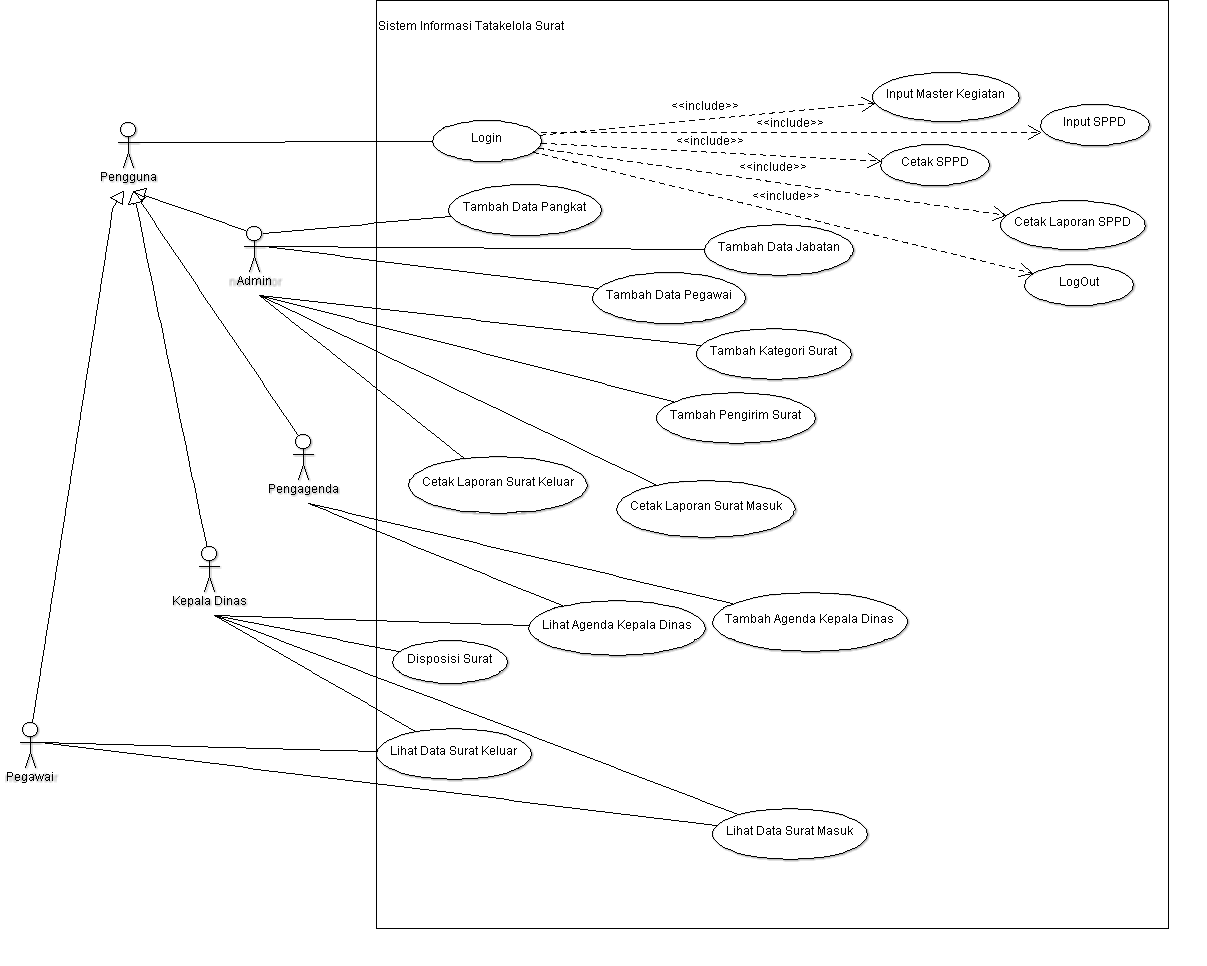
\includegraphics [height=8cm, width=10cm]{konten/gambar/UML/UseCaseDiagram2.png}
		\caption{Use Case Sistem Usulan}
		\label{UseCaseSistemUsulan}
	\end{figure}
	
	\item Kebutuhan Pengguna Sistem\\
	adapun Kebutuhan Pengguna sistem dapat dilihat pada \pic~\ref{AktorSistemSurat}.
		\begin{figure}
		\centering
		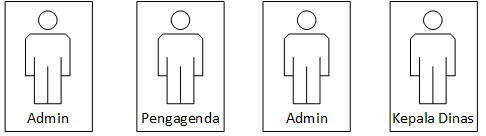
\includegraphics [height=3cm, width=4cm]{konten/gambar/AktorSistemSurat.png}
		\caption{Aktor Sistem Surat}
		\label{AktorSistemSurat}
		\end{figure}
	
	berikut adalah tabel deskripsi tugas dari masing - masing aktor pada \tab~\ref{Useraktor}
	{\fontsize{10pt}{12pt}\selectfont
		\renewcommand\namaTabel{Deskripsi pengguna \textit{user} }
		\begin{longtable}{p{1cm} p{2cm} p{10cm}}
			\caption{\namaTabel}\\
			\label{Useraktor}\\
			\hline
			No. & User & Deskripsi \\ \hline
			\endfirsthead
			%
			\multicolumn{3}{c}%
			{{\bfseries Table \thetable\ Tabel lanjutan ...}} \\
			\hline
			No. & User & Deskripsi \\ \hline
			\endhead
			%
			1. & Admin &  Mengurus \textit{Backend} dari aplikasi  \\
			2. & Pengagenda &  Menginput Data Surat Masuk dan Keluar. \\
			3. & Pegawai & Menerima Surat Masuk dan Keluar \\ 
			4. & Kepala Dinas & Menyetujui dan Mendisposisi Surat Divisi Lain \\ \hline
			%--------------------------------------------------------------------%
			
	\end{longtable}}

	\item Kebutuhan data dalam dalam pengembangan sistem antara lain :
	\begin{enumerate}
		\item data surat
		data surat yang diperlukan antara lain :
		nomer agenda, kategori surat, nomer surat, pengirim surat , perihal surat, isi ringkas dan keterangan surat.
		
		\item data pengguna
		sedangkan data pengguna yang dibutuhkan adalah sebagai berikut :
		nip, nama, golongan, jabatan, alamat dan email.
	\end{enumerate}

	\item Analisa Fitur dan Konten
	
	Adapun fitur dan konten yang terdapat pada aplikasi ini adalah:
	\begin{enumerate}
		\item mengelola data user
		fitur ini dibuat untuk admin yang dapat digunakan untuk menambahkan data user, menghapus data user dan mengesedit data user.
		\item menamhakan data surat
		fitur ini dibuat untuk pengagenda untuk menambahkan data surat masuk dan keluar
		\item menu disposisi
		menu ini dibuat untuk digunakan oleh kepala dinas dan pegawai agar bisa mendisposisikan surat ditingkat instansi.
		\item menu laporan
		menu ini dibuat untuk seluruh pengguna agar bisa mencetak laporan surat masuk dan keluar yang dibutuhkan.
		\item menu SPPD
		menu ini dibuat untuk kepala dinas dan pegawai agar dapat menerbitkan surat perintah perjalanan dinas ditingkat instansi.
	\end{enumerate}
\end{enumerate}

\section{\textit{Class Diagram}}

berikut merupakan desaign dari \textit{class diagram} yang diusulkan dalam sistem tatakelola surat

\section{Perancangan \textit{Database}}

Perancangan \textit{database} digunakan agar  setiap \textit{field} data  yang  mempunyai relasi dapat saling terhubung pada tabel \textit{database}. Perancangan tabel database pada sistem informasi tatakelola surat ini terdiri dari :

\begin{enumerate}
	\item tabel tb\_pegawai
	
	Nama \textit{Database} : Sistasur
	
	Nama tabel : tb\_pegawai
	
	\textit{Field} Kunci : id\_user
	
	Rancangan tabel tb\_pegawai dapat dilihat pada \tab~\ref{tb_pegawai}
	
	{\fontsize{10pt}{12pt}\selectfont
		\begin{longtable}{p{4cm}p{4cm}p{4cm}}
			\caption{Perancangan tabel pegawai}
			\label{tb_pegawai}\\
			\hline
			\textbf{Nama \textit{Field}} & \textbf{\textit{Type Data}} & \textbf{Panjang Data} \\ \hline
			\endfirsthead
			%
			\multicolumn{3}{c}%
			{{\bfseries Table \thetable\ continued from previous page}} \\
			\hline
			\textbf{Nama Field} & Type Data & Panjang Data \\ \hline
			\endhead
			%
			\textit{id\_user}             & \textit{int}       & 8            \\
			nip                 & \textit{varchar}   & 30           \\
			nama\_lengkap        & \textit{varchar}   & 60           \\
			golongan            & \textit{int}       & 8            \\
			jabatan             & \textit{int}       & 8            \\
			alamat              & \textit{text}      & -            \\
			no\_telp             & \textit{varchar}   & 15           \\
			\textit{email}               & \textit{varchar}   & 50           \\
			\textit{username}            & \textit{varchar}   & 40           \\
			\textit{password}            & \textit{varchar}   & 40           \\
			level\_user          & \textit{int}       & 1    \\\hline       
	\end{longtable}}
	
	
	
	
	\item tabel tb\_golongan
	
	Nama \textit{Database} : Sistasur
	
	Nama tabel : tb\_golongan
	
	\textit{Field} Kunci : id\_golongan
	
	Rancangan tabel tb\_pegawai dapat dilihat pada \tab~\ref{tb_golongan}
		
	{\fontsize{10pt}{12pt}\selectfont
		\begin{longtable}{p{4cm}p{4cm}p{4cm}}
			\caption{tabel golongan}
			\label{tb_golongan}\\
			\hline
			\textbf{Nama \textit{Field}} & \textbf{\textit{Type Data}} & \textbf{Panjang Data} \\ \hline
			\endfirsthead
			%
			\multicolumn{3}{c}%
			{{\bfseries Table \thetable\ continued from previous page}} \\
			\hline
			\textbf{Nama Field} & Type Data & Panjang Data \\ \hline
			\endhead
			%
			id\_golongan             & \textit{int}       & 8            \\
			kode\_golongan                 & \textit{varchar}   & 15           \\
			nama\_golongan        & \textit{varchar}   & 50           \\
			alamat              & \textit{text}      & -            \\\hline
	\end{longtable}}


	\item tabel tb\_jabatan
	
	Nama \textit{Database} : Sistasur
	
	Nama tabel : tb\_jabatan
	
	\textit{Field} Kunci : id\_jabatan
	
	Rancangan tabel tb\_jabatan dapat dilihat pada \tab~\ref{tb_jabatan}
	
	{\fontsize{10pt}{12pt}\selectfont
		\begin{longtable}{p{4cm}p{4cm}p{4cm}}
			\caption{Perancangan tabel jabatan}
			\label{tb_jabatan}\\
			\hline
			\textbf{Nama \textit{Field}} & \textbf{\textit{Type Data}} & \textbf{Panjang Data} \\ \hline
			\endfirsthead
			%
			\multicolumn{3}{c}%
			{{\bfseries Table \thetable\ continued from previous page}} \\
			\hline
			\textbf{Nama Field} & Type Data & Panjang Data \\ \hline
			\endhead
			%
			id\_jabatan             & \textit{int}       & 8            \\
			nama\_jabatan        & \textit{varchar}   & 100           \\
			uraian            & \textit{text}       & -            \\
			jabatan             & \textit{int}       & 8            \\
			kode\_surat              & \textit{varchar}      & 30            \\
			level\_jabatan             & \textit{enum}   & '0','2','3','4','5'           \\
			\textit{parent\_jabatan}               & \textit{int}   & 8           \\
			\hline       
	\end{longtable}}
	
	
	\item tabel tb\_agenda
	
	Nama \textit{Database} : Sistasur
	
	Nama tabel : tb\_agenda
	
	\textit{Field} Kunci : id\_agenda
	
	Rancangan tabel tb\_jabatan dapat dilihat pada \tab~\ref{tb_agenda}
	
	{\fontsize{10pt}{12pt}\selectfont
		\begin{longtable}{p{4cm}p{4cm}p{4cm}}
			\caption{Perancangan tabel agenda}
			\label{tb_agenda}\\
			\hline
			\textbf{Nama \textit{Field}} & \textbf{\textit{Type Data}} & \textbf{Panjang Data} \\ \hline
			\endfirsthead
			%
			\multicolumn{3}{c}%
			{{\bfseries Table \thetable\ continued from previous page}} \\
			\hline
			\textbf{Nama Field} & Type Data & Panjang Data \\ \hline
			\endhead
			%
			id\_agenda             & \textit{int}       & 8            \\
			no\_agenda        & \textit{int}   & 10           \\
			tgl\_start            & \textit{date}       & -            \\
			jam\_start             & \textit{varchar}       & 10            \\
			tgl\_end              & \textit{date}      & -            \\
			jam\_end             & \textit{varchar}       & 10            \\
			perihal\_acara		& \textit{varchar} 		& 200 			\\
			tempat\_acara		& \textit{varchar} 		& 150			\\
			keterangan 			& \textit{text}			& -				\\
			user\_input             & \textit{int}       & 8            \\        \\
			\hline       
	\end{longtable}}

	
	\item tabel tb\_disposisi\_surat
	
	Nama \textit{Database} : Sistasur
	
	Nama tabel : tb\_disposisi\_surat
	
	\textit{Field} Kunci : id\_disposisi
	
	Rancangan tabel tb\_disposisi\_surat dapat dilihat pada \tab~\ref{tb_disposisi_surat}
	
	{\fontsize{10pt}{12pt}\selectfont
		\begin{longtable}{p{4cm}p{4cm}p{4cm}}
			\caption{Perancangan tabel disposisi surat}
			\label{tb_disposisi_surat}\\
			\hline
			\textbf{Nama \textit{Field}} & \textbf{\textit{Type Data}} & \textbf{Panjang Data} \\ \hline
			\endfirsthead
			%
			\multicolumn{3}{c}%
			{{\bfseries Table \thetable\ continued from previous page}} \\
			\hline
			\textbf{Nama Field} & Type Data & Panjang Data \\ \hline
			\endhead
			%
			id\_disposisi             & \textit{int}       & 8            \\
			input\_diteruskan        & \textit{enum}   & '1','2'           \\
			catatan           & \textit{text}       & -            \\
			id\_surat\_in             & \textit{int}       & 8            \\
			id\_surat\_in             & \textit{int}       & 8            \\ 
			\hline       
		\end{longtable}}
	
	\item tabel tb\_disp\_detail\_perintah
	
	
	Nama \textit{Database} : Sistasur
	
	Nama tabel : tb\_disp\_detail\_perintah
	
	\textit{Field} Kunci : id\_disp\_detail\_perintah
	
	Rancangan tabel tb\_disp\_detail\_perintah dapat dilihat pada \tab~\ref{disp_detail_perintah}
	
	{\fontsize{10pt}{12pt}\selectfont
		\begin{longtable}{p{4cm}p{4cm}p{4cm}}
			\caption{Perancangan tabel disposisi detail perintah}
			\label{disp_detail_perintah}\\
			\hline
			\textbf{Nama \textit{Field}} & \textbf{\textit{Type Data}} & \textbf{Panjang Data} \\ \hline
			\endfirsthead
			%
			\multicolumn{3}{c}%
			{{\bfseries Table \thetable\ continued from previous page}} \\
			\hline
			\textbf{Nama Field} & Type Data & Panjang Data \\ \hline
			\endhead
			%
			id\_disp\_detail\_perintah            & \textit{int}       & 8            \\
			input\_perintah        & \textit{int}       & 8            \\
			id\_disposisi          & \textit{int}       & 8            \\
			\hline       
	\end{longtable}}
	
	
	\item tabel tb\_disp\_detail\_tujuan
	
	
	Nama \textit{Database} : Sistasur
	
	Nama tabel : tb\_disp\_detail\_tujuan
	
	\textit{Field} Kunci : id\_disp\_detail\_tujuan
	
	Rancangan tabel tb\_disp\_detail\_tujuan dapat dilihat pada \tab~\ref{tb_disp_detail_tujuan}
	
	{\fontsize{10pt}{12pt}\selectfont
		\begin{longtable}{p{4cm}p{4cm}p{4cm}}
			\caption{Perancangan tabel disp detail tujuan}
			\label{tb_disp_detail_tujuan}\\
			\hline
			\textbf{Nama \textit{Field}} & \textbf{\textit{Type Data}} & \textbf{Panjang Data} \\ \hline
			\endfirsthead
			%
			\multicolumn{3}{c}%
			{{\bfseries Table \thetable\ continued from previous page}} \\
			\hline
			\textbf{Nama Field} & Type Data & Panjang Data \\ \hline
			\endhead
			%
			id\_disp\_detail\_tujuan            & \textit{int}       & 8            \\
			id\_jabatan        & \textit{int}       & 8            \\
			id\_user          & \textit{int}       & 8            \\
			id\_disposisi          & \textit{int}       & 8            \\
			\hline       
	\end{longtable}}

	\item tabel tb\_disp\_perintah
	
	
	Nama \textit{Database} : Sistasur
	
	Nama tabel : tb\_disp\_perintah
	
	\textit{Field} Kunci : id\_disp\_perintah
	
	Rancangan tabel tb\_disp\_perintah dapat dilihat pada \tab~\ref{tb_disp_perintah}
	
	{\fontsize{10pt}{12pt}\selectfont
		\begin{longtable}{p{4cm}p{4cm}p{4cm}}
			\caption{Perancangan tabel disposisi perintah}
			\label{tb_disp_perintah}\\
			\hline
			\textbf{Nama \textit{Field}} & \textbf{\textit{Type Data}} & \textbf{Panjang Data} \\ \hline
			\endfirsthead
			%
			\multicolumn{3}{c}%
			{{\bfseries Table \thetable\ continued from previous page}} \\
			\hline
			\textbf{Nama Field} & Type Data & Panjang Data \\ \hline
			\endhead
			%
			id\_disp\_perintah            & \textit{int}       & 8            \\
			isi\_perintah        & \textit{varchar}       & 100            \\
			ket          & \textit{text}       & -            \\
			\hline       
	\end{longtable}}


	\item tabel tb\_kategori\_surat
	
	Nama \textit{Database} : Sistasur
	
	Nama tabel : tb\_kategori\_surat
	
	\textit{Field} Kunci : id\_kategori
	
	Rancangan tabel tb\_kategori\_surat dapat dilihat pada \tab~\ref{tb_kategori_surat}
	
	{\fontsize{10pt}{12pt}\selectfont
		\begin{longtable}{p{4cm}p{4cm}p{4cm}}
			\caption{Perancangan tabel kategori surat}
			\label{tb_kategori_surat}\\
			\hline
			\textbf{Nama \textit{Field}} & \textbf{\textit{Type Data}} & \textbf{Panjang Data} \\ \hline
			\endfirsthead
			%
			\multicolumn{3}{c}%
			{{\bfseries Table \thetable\ continued from previous page}} \\
			\hline
			\textbf{Nama Field} & Type Data & Panjang Data \\ \hline
			\endhead
			%
			id\_kategori            & \textit{int}       & 8            \\
			kode\_kategori        & \textit{varchar}       & 15            \\
			nama\_kategori          & \textit{varchar}       & 15            \\
			uraian 				& \textit{text}				& -		\\
			\hline       
	\end{longtable}}


	\item tabel tb\_pengirim\_surat
	
	
	Nama \textit{Database} : Sistasur
	
	Nama tabel : tb\_pengirim\_surat
	
	\textit{Field} Kunci : id\_pengirim
	
	Rancangan tabel tb\_pengirim\_surat dapat dilihat pada \tab~\ref{tb_pengirim_surat}
	
	{\fontsize{10pt}{12pt}\selectfont
		\begin{longtable}{p{4cm}p{4cm}p{4cm}}
			\caption{Perancangan tabel pengirim surat}
			\label{tb_pengirim_surat}\\
			\hline
			\textbf{Nama \textit{Field}} & \textbf{\textit{Type Data}} & \textbf{Panjang Data} \\ \hline
			\endfirsthead
			%
			\multicolumn{3}{c}%
			{{\bfseries Table \thetable\ continued from previous page}} \\
			\hline
			\textbf{Nama Field} & Type Data & Panjang Data \\ \hline
			\endhead
			%
			id\_pengirim            & \textit{int}       & 8            \\
			nama\_pengirim        & \textit{varchar}       & 70            \\
			uraian 				& \textit{text}				& -		\\
			\hline       
	\end{longtable}}

	\item tabel tb\_sppd
	
	Nama \textit{Database} : Sistasur
	
	Nama tabel : tb\_sppd
	
	\textit{Field} Kunci : id\_sppd
	
	Rancangan tabel tb\_sppd dapat dilihat pada \tab~\ref{tb_sppd}
	
	{\fontsize{10pt}{12pt}\selectfont
		\begin{longtable}{p{4cm}p{4cm}p{4cm}}
			\caption{Perancangan tabel tb\_sppd}
			\label{tb_sppd}\\
			\hline
			\textbf{Nama \textit{Field}} & \textbf{\textit{Type Data}} & \textbf{Panjang Data} \\ \hline
			\endfirsthead
			%
			\multicolumn{3}{c}%
			{{\bfseries Table \thetable\ continued from previous page}} \\
			\hline
			\textbf{Nama Field} & Type Data & Panjang Data \\ \hline
			\endhead
			%
			id\_sppd            & \textit{int}       	& 8     \\
			no\_sppd        	& \textit{varchar}      & 50    \\
			pejabat				& \textit{int}			& 8	    \\
			maksud				& \textit{text}			& -		\\
			kenderaan			& \textit{varchar}		& 60    \\
			tempat\_berangkat	& \textit{varchar}		& 60	\\
			tujuan\_tujuan		& \textit{varchar}		& 60	\\
			tgl\_berangkat		& \textit{date} 		& -		\\
			tgl\_kembali		& \textit{date} 		& -		\\
			keberangkatan		& \textit{int}	 		& 8		\\
			tgl\_sppd			& \textit{date} 		& -		\\
			ttd					& \textit{int}			& 8		\\
			keterangan 			& \textit{text}			& - 	\\
			tgl\_catat 			& \textit{date}			& - 	\\
			user\_input 		& \textit{int}			& 8 	\\\hline  
	\end{longtable}}

	
	\item tabel tb\_sppd\_dasar
	
	Nama \textit{Database} : Sistasur
	
	Nama tabel : tb\_sppd\_dasar
	
	\textit{Field} Kunci : id\_dasar
	
	Rancangan tabel tb\_sppd\_dasar dapat dilihat pada \tab~\ref{tb_sppd_dasar}
	
	{\fontsize{10pt}{12pt}\selectfont
		\begin{longtable}{p{4cm}p{4cm}p{4cm}}
			\caption{Perancangan tabel tb\_sppd\_dasar}
			\label{tb_sppd_dasar}\\
			\hline
			\textbf{Nama \textit{Field}} & \textbf{\textit{Type Data}} & \textbf{Panjang Data} \\ \hline
			\endfirsthead
			%
			\multicolumn{3}{c}%
			{{\bfseries Table \thetable\ continued from previous page}} \\
			\hline
			\textbf{Nama Field} & Type Data & Panjang Data \\ \hline
			\endhead
			%
			id\_dasar           & \textit{int}       	& 8     \\
			uraian        		& \textit{text}      	& -    \\
			id\_sppd			& \textit{int}			& 8	    \\
			\hline  
	\end{longtable}}
	
	
	\item tabel tb\_sppd\_kegiatan
	
	Nama \textit{Database} : Sistasur
	
	Nama tabel : tb\_sppd\_kegiatan
	
	\textit{Field} Kunci : id\_dasar
	
	Rancangan tabel tb\_sppd\_kegiatan dapat dilihat pada \tab~\ref{tb_sppd_kegiatan}
	
	{\fontsize{10pt}{12pt}\selectfont
		\begin{longtable}{p{4cm}p{4cm}p{4cm}}
			\caption{Perancangan tabel tb\_sppd}
			\label{tb_sppd_kegiatan}\\
			\hline
			\textbf{Nama \textit{Field}} & \textbf{\textit{Type Data}} & \textbf{Panjang Data} \\ \hline
			\endfirsthead
			%
			\multicolumn{3}{c}%
			{{\bfseries Table \thetable\ continued from previous page}} \\
			\hline
			\textbf{Nama Field} & Type Data & Panjang Data \\ \hline
			\endhead
			%
			id\_keg           		& \textit{int}       		& 8     \\
			kode\_rek        		& \textit{varchar}      	& 50    \\
			nama\_keg				& \textit{varchar}			& 200	\\
			pptk 					& \textit{int}				& 8		\\
			bendahara 				& \textit{int}				& 8		\\
			jumlah\_anggaran 		& \textit{double}			& -		\\
			user\_input 			& \textit{int}				& 8		\\
			\hline  
	\end{longtable}}


\item tabel tb\_sppd\_lap\_hal

Nama \textit{Database} : Sistasur

Nama tabel : tabel tb\_sppd\_lap\_hal

\textit{Field} Kunci : id\_lap\_hal

Rancangan tabel tb\_sppd\_lap\_hal dapat dilihat pada \tab~\ref{tb_sppd_lap_hal}

{\fontsize{10pt}{12pt}\selectfont
	\begin{longtable}{p{4cm}p{4cm}p{4cm}}
		\caption{Perancangan tabel tb\_sppd}
		\label{tb_sppd_lap_hal}\\
		\hline
		\textbf{Nama \textit{Field}} & \textbf{\textit{Type Data}} & \textbf{Panjang Data} \\ \hline
		\endfirsthead
		%
		\multicolumn{3}{c}%
		{{\bfseries Table \thetable\ continued from previous page}} \\
		\hline
		\textbf{Nama Field} & Type Data & Panjang Data \\ \hline
		\endhead
		%
		id\_lap\_hal           	& \textit{int}       	& 8   \\
		uraian	        		& \textit{text}      	& -   \\
		id\_kegiatan			& \textit{int}			& 8	  \\
		\hline  
\end{longtable}}


	\item tabel tb\_sppd\_lap\_ttd
	
	Nama \textit{Database} : Sistasur
	
	Nama tabel : tb\_sppd\_lap\_ttd
	
	\textit{Field} Kunci : id\_lap\_ttd 
	
	Rancangan tabel tb\_sppd\_lap\_ttd dapat dilihat pada \tab~\ref{id_lap_ttd}
	
	{\fontsize{10pt}{12pt}\selectfont
		\begin{longtable}{p{4cm}p{4cm}p{4cm}}
			\caption{Perancangan tabel tb\_sppd\_lap\_ttd}
			\label{id_lap_ttd}\\
			\hline
			\textbf{Nama \textit{Field}} & \textbf{\textit{Type Data}} & \textbf{Panjang Data} \\ \hline
			\endfirsthead
			%
			\multicolumn{3}{c}%
			{{\bfseries Table \thetable\ continued from previous page}} \\
			\hline
			\textbf{Nama Field} & Type Data & Panjang Data \\ \hline
			\endhead
			%
			id\_lap\_ttd           	& \textit{int}       	& 8   \\
			pgw\_mengetahui	        		& \textit{int}      	& 8   \\
			tgl\_surat			& \textit{date}			& -	  \\
			id\_kegiatan			& \textit{int}			& 8	  \\
			\hline  
	\end{longtable}}
	
	
\item tabel tb\_sppd\_pelaksana

Nama \textit{Database} : Sistasur

Nama tabel : tb\_sppd\_pelaksana

\textit{Field} Kunci : id\_pelaksana 

Rancangan tabel tb\_sppd\_pelaksana dapat dilihat pada \tab~\ref{id_pelaksana}

{\fontsize{10pt}{12pt}\selectfont
	\begin{longtable}{p{4cm}p{4cm}p{4cm}}
		\caption{Perancangan tabel tb\_sppd\_pelaksana}
		\label{id_pelaksana}\\
		\hline
		\textbf{Nama \textit{Field}} & \textbf{\textit{Type Data}} & \textbf{Panjang Data} \\ \hline
		\endfirsthead
		%
		\multicolumn{3}{c}%
		{{\bfseries Table \thetable\ continued from previous page}} \\
		\hline
		\textbf{Nama Field} & Type Data & Panjang Data \\ \hline
		\endhead
		%
		id\_pelaksana           & \textit{int}       	& 8   \\
		pegawai        			& \textit{int}      	& 8   \\
		uraian					& \textit{text}			& -	  \\
		id\_sppd			& \textit{int}			& 8	  \\
		\hline  
\end{longtable}}

\item tabel tb\_sppd\_pengikut

Nama \textit{Database} : Sistasur

Nama tabel : tb\_sppd\_pengikut

\textit{Field} Kunci : id\_pengikut 

Rancangan tabel tb\_sppd\_pengikut dapat dilihat pada \tab~\ref{tb_sppd_pengikut}

{\fontsize{10pt}{12pt}\selectfont
	\begin{longtable}{p{4cm}p{4cm}p{4cm}}
		\caption{Perancangan tabel tb\_sppd\_pengikut}
		\label{tb_sppd_pengikut}\\
		\hline
		\textbf{Nama \textit{Field}} & \textbf{\textit{Type Data}} & \textbf{Panjang Data} \\ \hline
		\endfirsthead
		%
		\multicolumn{3}{c}%
		{{\bfseries Table \thetable\ continued from previous page}} \\
		\hline
		\textbf{Nama Field} & Type Data & Panjang Data \\ \hline
		\endhead
		%
		id\_pengikut            & \textit{int}       	& 8   \\
		pegawai        			& \textit{int}      	& 8   \\
		uraian					& \textit{text}			& -	  \\
		id\_pelaksana			& \textit{int}			& 8	  \\
		id\_sppd				& \textit{int}			& 8	  \\
		\hline  
\end{longtable}}

\item tabel tb\_surat\_keluar

Nama \textit{Database} : Sistasur

Nama tabel : tb\_surat\_keluar

\textit{Field} Kunci : id\_surat\_out

Rancangan tabel tb\_surat\_keluar dapat dilihat pada \tab~\ref{tb_surat_keluar}

{\fontsize{10pt}{12pt}\selectfont
	\begin{longtable}{p{4cm}p{4cm}p{4cm}}
		\caption{Perancangan tabel tb\_surat\_keluar}
		\label{tb_surat_keluar}\\
		\hline
		\textbf{Nama \textit{Field}} & \textbf{\textit{Type Data}} & \textbf{Panjang Data} \\ \hline
		\endfirsthead
		%
		\multicolumn{3}{c}%
		{{\bfseries Table \thetable\ continued from previous page}} \\
		\hline
		\textbf{Nama Field} & Type Data & Panjang Data \\ \hline
		\endhead
		%
		id\_surat\_out          	& \textit{int}       		& 8  \\
		no\_agenda        			& \textit{int}      		& 10  \\
		kategori					& \textit{int}				& 8	  \\
		no\_surat					& \textit{varchar}			& 70  \\
		tgl\_surat					& \textit{date}				& -	  \\
		perihal						& \textit{varchar}			& 70  \\
		isi\_ringkas				& \textit{text}				& -	  \\
		tujuan						& \textit{int}				& -	  \\
		pengelolah					& \textit{varchar}			& 30  \\
		file\_surat					& \textit{varchar}			& 50  \\
		keterangan					& \textit{text}				& -	  \\
		tgl\_catat					& \textit{date}				& -	  \\
		user\_input					& \textit{int}				& 8	  \\
		\hline  
\end{longtable}}

\item tabel tb\_surat\_masuk

Nama \textit{Database} : Sistasur

Nama tabel : tb\_surat\_masuk

\textit{Field} Kunci : id\_surat\_in

Rancangan tabel tb\_surat\_keluar dapat dilihat pada \tab~\ref{tb_surat_masuk}

{\fontsize{10pt}{12pt}\selectfont
	\begin{longtable}{p{4cm}p{4cm}p{4cm}}
		\caption{Perancangan tabel tb\_surat\_keluar}
		\label{tb_surat_masuk}\\
		\hline
		\textbf{Nama \textit{Field}} & \textbf{\textit{Type Data}} & \textbf{Panjang Data} \\ \hline
		\endfirsthead
		%
		\multicolumn{3}{c}%
		{{\bfseries Table \thetable\ continued from previous page}} \\
		\hline
		\textbf{Nama Field} & Type Data & Panjang Data \\ \hline
		\endhead
		%
		id\_surat\_in          		& \textit{int}       		& 8  \\
		no\_agenda        			& \textit{int}      		& 10  \\
		kategori					& \textit{int}				& 8	  \\
		input\_pengirim				& \textit{enum}				& '1','2'	  \\
		pengirim					& \textit{varchar}			& 150  \\
		no\_surat					& \textit{varchar}			& 70  \\
		tgl\_surat					& \textit{date}				& -	  \\
		perihal						& \textit{varchar}			& 70  \\
		isi\_ringkas				& \textit{text}				& -	  \\
		file\_surat					& \textit{varchar}			& 50  \\
		sifat\_surat				& \textit{enum}				& 'Sangat Segera','Segera','Rahasia','Penting'	  \\
		keterangan					& \textit{text}				& -  \\
		tgl\_catat					& \textit{date}				& -	  \\
		user\_input					& \textit{int}				& 8	  \\
		\hline  
\end{longtable}}


\item tabel tb\_tujuan\_surat

Nama \textit{Database} : Sistasur

Nama tabel : tb\_tujuan\_surat

\textit{Field} Kunci : id\_tujuan

Rancangan tabel tb\_tujuan\_surat dapat dilihat pada \tab~\ref{tb_tujuan_surat}

{\fontsize{10pt}{12pt}\selectfont
	\begin{longtable}{p{4cm}p{4cm}p{4cm}}
		\caption{Perancangan tabel tb\_tujuan\_surat}
		\label{tb_tujuan_surat}\\
		\hline
		\textbf{Nama \textit{Field}} & \textbf{\textit{Type Data}} & \textbf{Panjang Data} \\ \hline
		\endfirsthead
		%
		\multicolumn{3}{c}%
		{{\bfseries Table \thetable\ continued from previous page}} \\
		\hline
		\textbf{Nama Field} & Type Data & Panjang Data \\ \hline
		\endhead
		%
		id\_tujuan          			& \textit{int}       		& 8  \\
		alamat\_tujuan        			& \textit{text}      		& -  \\
		uraian							& \textit{text}				& -	  \\
		\hline  
\end{longtable}}
	
\end{enumerate}

\section{Perancangan Antarmuka}

\begin{enumerate}
	
	\item Desain Antar Muka Admin
	
	\begin{enumerate}
		
		\item	Halaman Login sistem
		
		Halaman Login dapat dilihat pada \pic~\ref{HalamanLogin}.
		
		Pada halaman ini terdapat 2 input \textit{type} yaitu :
		\begin{enumerate}
			\item inputan untuk memasukkan \textit{username}
			\item inputan untuk memasukkan \textit{password}
		\end{enumerate}
		lalu selanjutnya akan masuk ke halaman dashboard.
		\begin{figure}
			\centering
			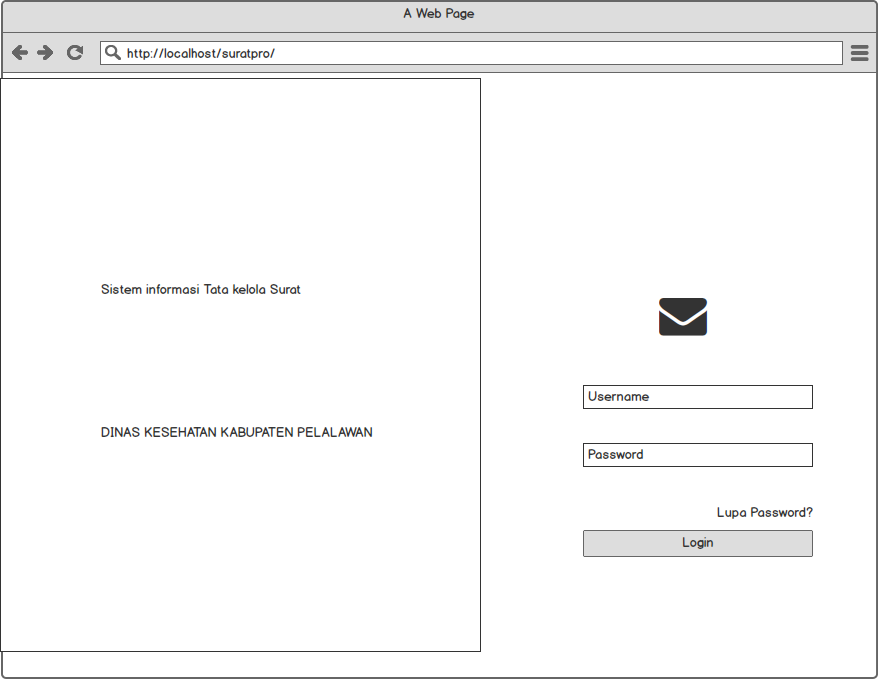
\includegraphics [height= 7cm, width=9cm]{konten/gambar/WireFrameSistemSurat/Admin/HalamanLogin.png}
			\caption{Halaman Login}
			\label{HalamanLogin}
		\end{figure}
		
		\item Dashboard
		
		Halaman dashboard dapat dilihat pada \pic\ref{HalamanDashboard1}
		
		pada halaman dashboard, terdapat beberapa menu, sesuai level user yang login, dalam hal ini adalah admin. Pada level admin, terdapat menu Agenda, Surat masuk , cetak laporan dan lain-lain. 
		\begin{figure}
			\centering
			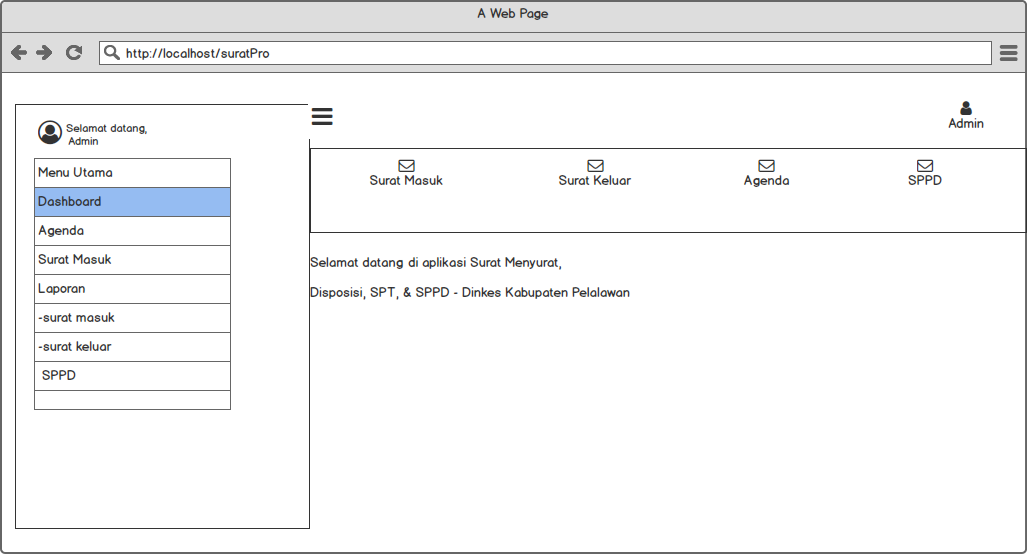
\includegraphics [height= 7cm, width=11cm]{konten/gambar/WireFrameSistemSurat/Admin/DashBoard.png}
			\caption{Halaman Dashboard}
			\label{HalamanDashboard1}
		\end{figure}
		
		\item Menu Master Golongan
		
		Halaman Menu Master Golongan dapat dilihat pada \pic\ref{HalamanInputMasterGolongan}
		
		\begin{figure}
			\centering
			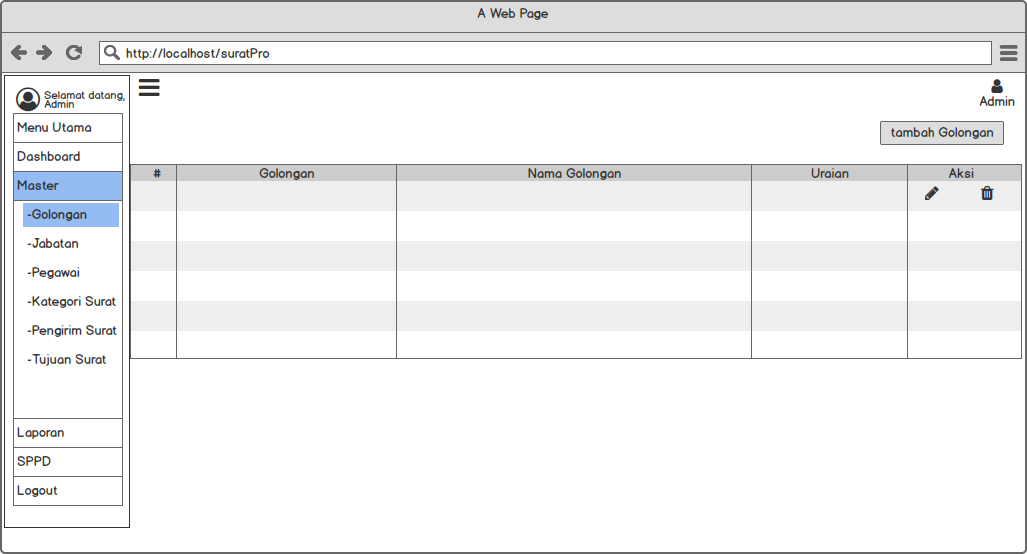
\includegraphics [height= 7cm, width=11cm]{konten/gambar/WireFrameSistemSurat/Admin/Mastergolongan.png}
			\caption{Halaman Input Master Golongan}
			\label{HalamanInputMasterGolongan}
		\end{figure}
		
		\item Menu Master Jabatan
		
		Halaman Input Master Jabatan dapat dilihat pada \pic\ref{HalamanInputMasterJabatan}
		
		\begin{figure}
			\centering
			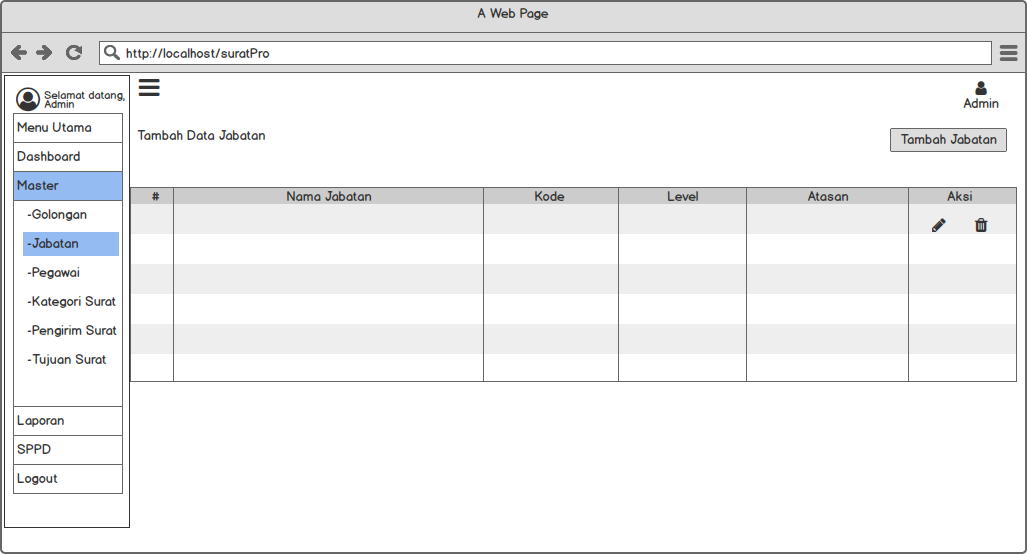
\includegraphics [height= 7cm, width=11cm]{konten/gambar/WireFrameSistemSurat/Admin/MasterJabatan.png}
			\caption{Halaman Input Master Jabatan}
			\label{HalamanInputMasterJabatan}
		\end{figure}
		
		\item Menu Master Pegawai
		
		Halaman Input Master Pegawai dapat dilihat pada \pic\ref{HalamanInputMasterPegawai}
		
		\begin{figure}
			\centering
			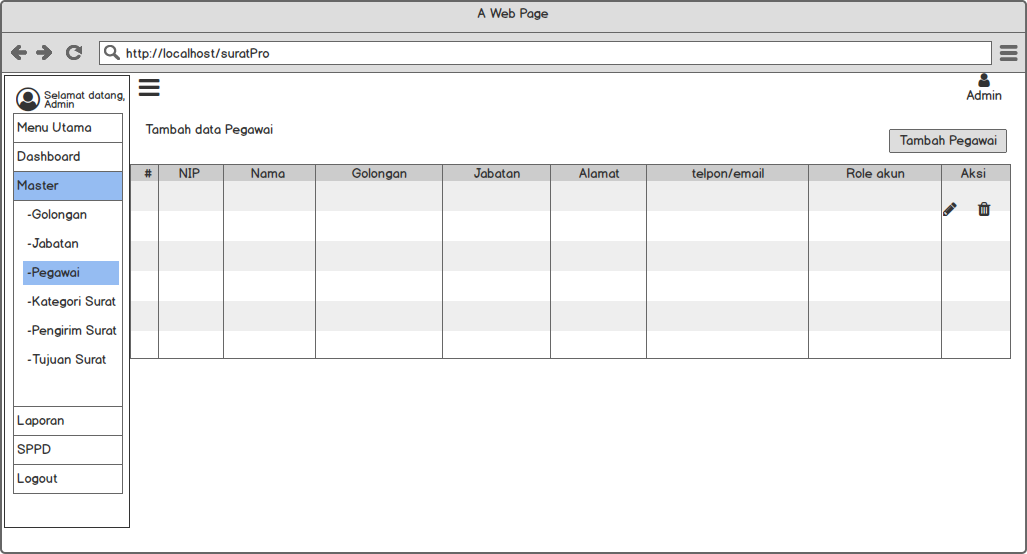
\includegraphics [height= 7cm, width=11cm]{konten/gambar/WireFrameSistemSurat/Admin/MasterPegawai.png}
			\caption{Halaman Input Master Pegawai}
			\label{HalamanInputMasterPegawai}
		\end{figure}
		
		\item Menu Master Kategori Surat
		
		Halaman Menu Master Kategori Surat dapat dilihat pada \pic\ref{HalamanInputKategoriSurat}
		
		\begin{figure}
			\centering
			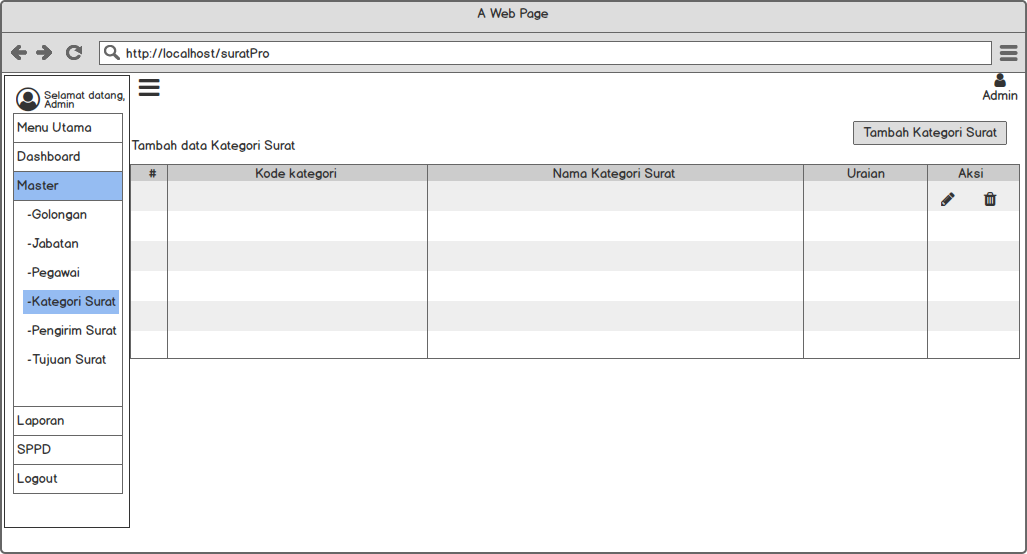
\includegraphics [height= 7cm, width=11cm]{konten/gambar/WireFrameSistemSurat/Admin/MasterKategoriSurat.png}
			\caption{Halaman Input Kategori Surat}
			\label{HalamanInputKategoriSurat}
		\end{figure}
		
		\item Menu Master Pengirim Surat
		
		Halaman Menu Master Pengirim Surat dapat dilihat pada \pic\ref{HalamanInputMasterPegawai}
		
		\begin{figure}
			\centering
			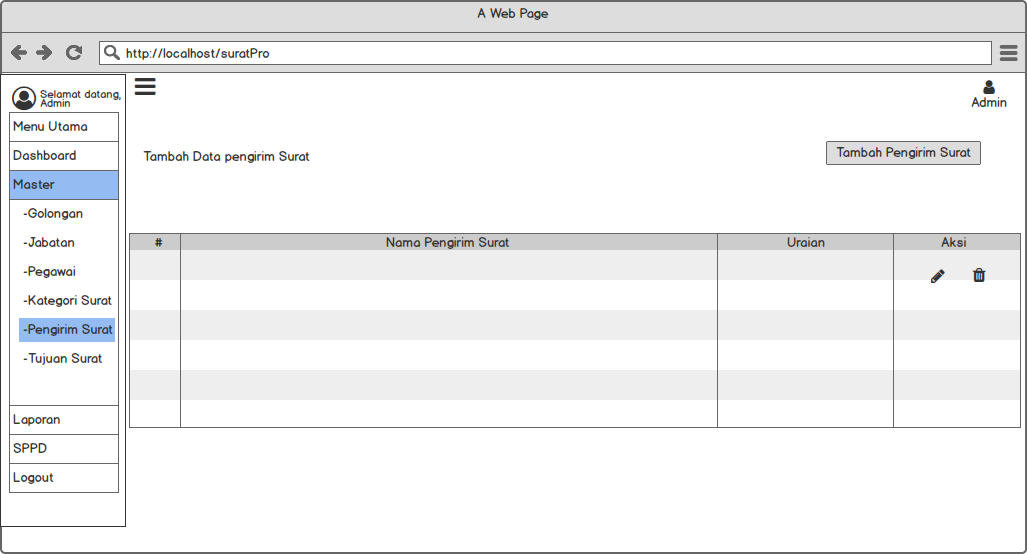
\includegraphics [height= 7cm, width=11cm]{konten/gambar/WireFrameSistemSurat/Admin/MasterPengirimSurat.png}
			\caption{Halaman Input Pengirim Surat}
			\label{HalamanInputPengirimSurat}
		\end{figure}
		
		\item Menu Master Tujuan Surat
		
		Halaman Menu Master Tujuan Surat dapat dilihat pada \pic\ref{HalamanInputTujuanSurat}
		
		\begin{figure}
			\centering
			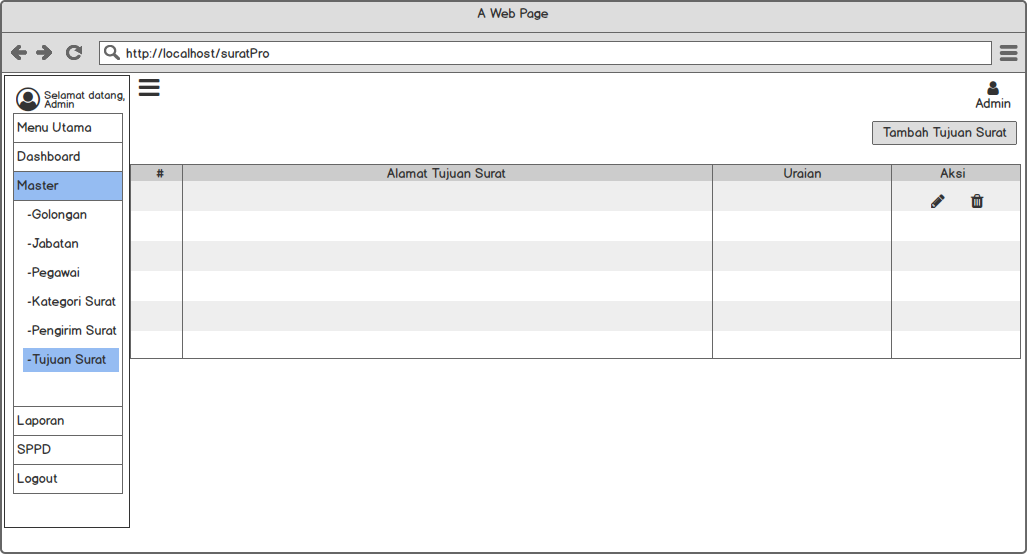
\includegraphics [height= 7cm, width=11cm]{konten/gambar/WireFrameSistemSurat/Admin/MasterTujuanSurat.png}
			\caption{Halaman Input Tujuan Surat}
			\label{HalamanInputTujuanSurat}
		\end{figure}
		
		\item Menu Laporan Surat Masuk
		
		Halaman Menu Laporan Surat Masuk  dapat dilihat pada \pic\ref{HalamanCetakLaporanSuratMasuk}
		
		\begin{figure}
			\centering
			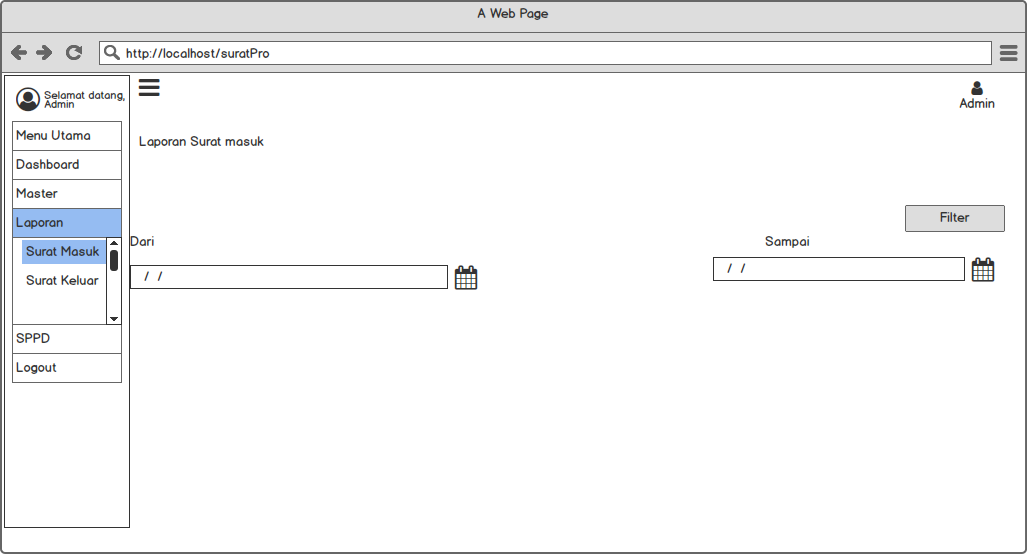
\includegraphics [height= 7cm, width=11cm]{konten/gambar/WireFrameSistemSurat/Admin/LaporanSuratMasuk.png}
			\caption{Halaman Cetak Laporan Surat Masuk}
			\label{HalamanCetakLaporanSuratMasuk}
		\end{figure}
		
		\item Menu Laporan Surat Keluar
		
		Halaman Menu Laporan Surat Keluar  dapat dilihat pada \pic\ref{HalamanCetakLaporanSuratKeluar}
		
		\begin{figure}
			\centering
			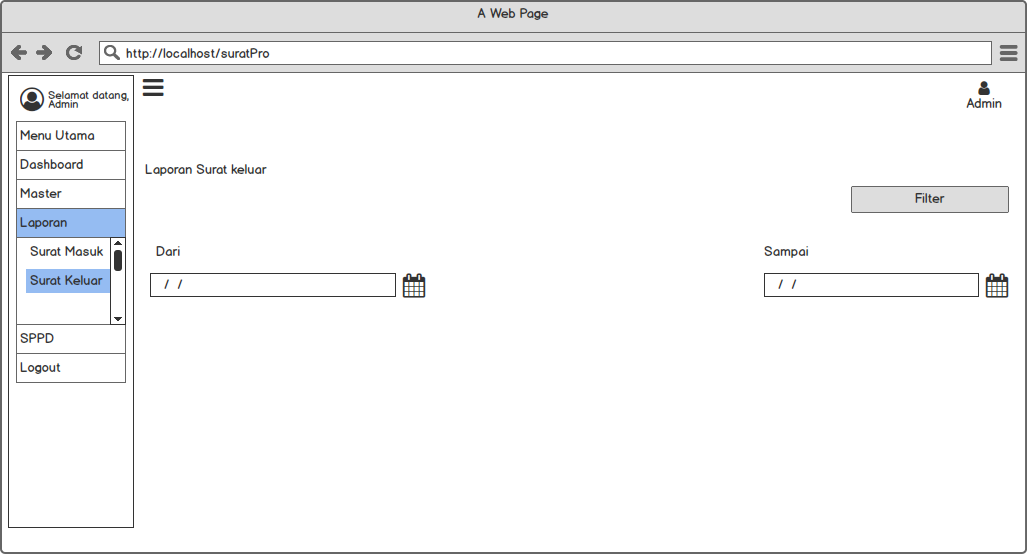
\includegraphics [height= 7cm, width=11cm]{konten/gambar/WireFrameSistemSurat/Admin/LaporanSuratKeluar.png}
			\caption{Halaman Cetak Laporan Surat Keluar}
			\label{HalamanCetakLaporanSuratKeluar}
		\end{figure}
		
		\item Menu SPPD Master Kegiatan
		
		Halaman Menu SPPD Master Kegiatan  dapat dilihat pada \pic\ref{HalamanLihatMasterSPPD}
		
		\begin{figure}
			\centering
			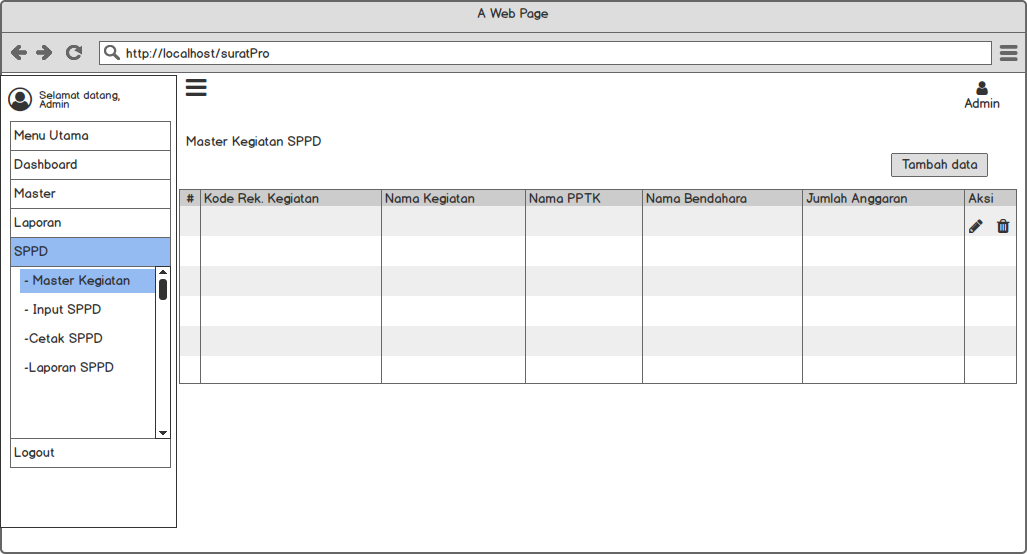
\includegraphics [height= 7cm, width=11cm]{konten/gambar/WireFrameSistemSurat/Admin/MasterkegiatanSPPD.png}
			\caption{Halaman Lihat Master SPPD}
			\label{HalamanLihatMasterSPPD}
		\end{figure}
		
		\item Menu SPPD Input SPPD
		
		Halaman Menu SPPD Input SPPD  dapat dilihat pada \pic\ref{HalamanInputMasterSPPD}
		
		\begin{figure}
			\centering
			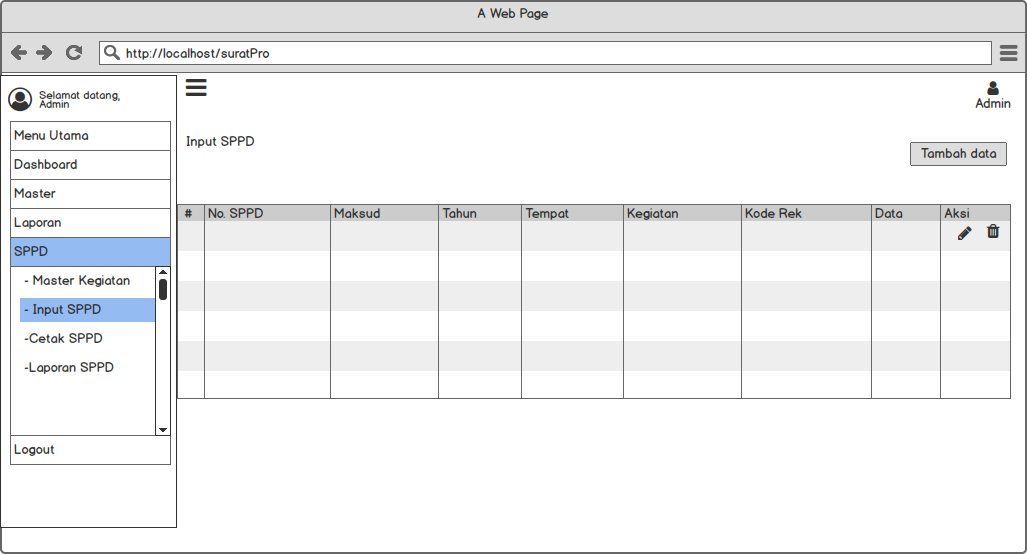
\includegraphics [height= 7cm, width=11cm]{konten/gambar/WireFrameSistemSurat/Admin/InputSPPD.png}
			\caption{Halaman Input Master SPPD}
			\label{HalamanInputMasterSPPD}
		\end{figure}
		
		\item Menu SPPD Cetak SPPD
		
		Halaman Menu SPPD Cetak SPPD  dapat dilihat pada \pic\ref{HalamanCetakSPPD}
		
		\begin{figure}
			\centering
			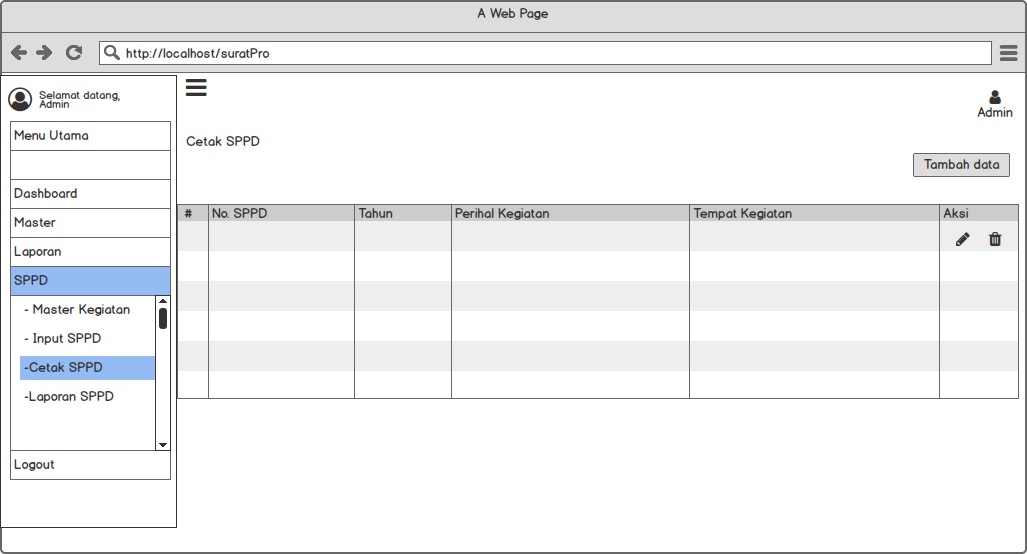
\includegraphics [height= 7cm, width=11cm]{konten/gambar/WireFrameSistemSurat/Admin/CetakSPPD.png}
			\caption{Halaman Cetak SPPD}
			\label{HalamanCetakSPPD}
		\end{figure}
		
		\item Menu Laporan SPPD
		
		Halaman Menu Laporan SPPD dapat dilihat pada \pic\ref{HalamanLihatLaporanSPPD}
		
		\begin{figure}
			\centering
			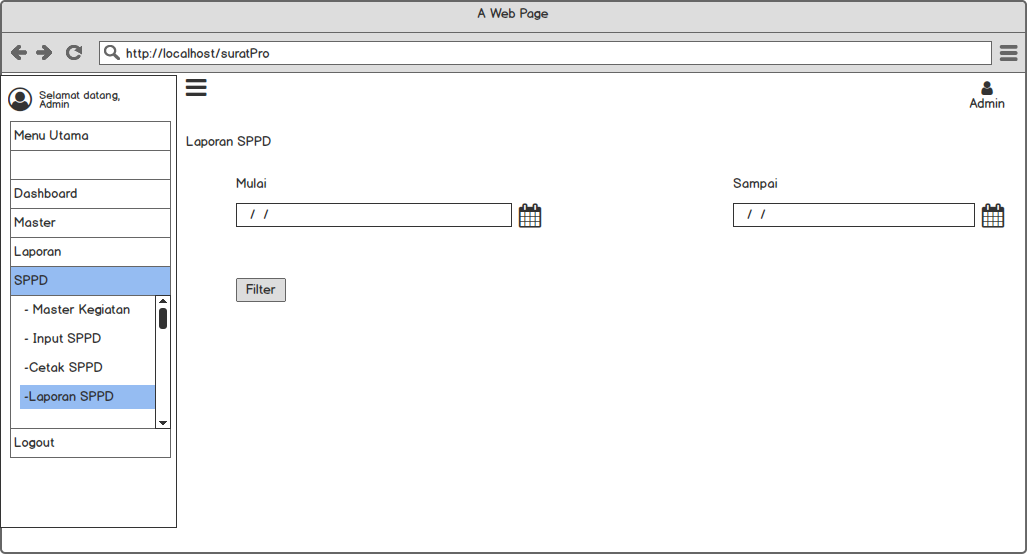
\includegraphics [height= 7cm, width=11cm]{konten/gambar/WireFrameSistemSurat/Admin/LaporanSPPD.png}
			\caption{Halaman Lihat Laporan SPPD}
			\label{HalamanLihatLaporanSPPD}
		\end{figure}
	\end{enumerate}
	
	\item Desagin Antar Muka Kadis
	
	\begin{enumerate}
		\item Dashboard
		
		Halaman Dashboard Kadis dapat dilihat pada \pic~\ref{HalamanDashboardKadis}.
		\begin{figure}
			\centering
			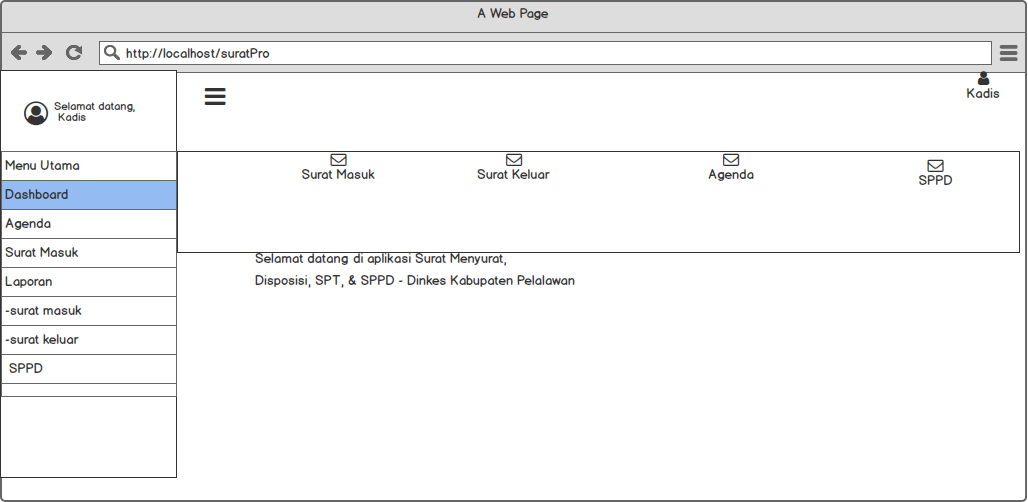
\includegraphics [height= 7cm, width=11cm]{konten/gambar/WireFrameSistemSurat/Kadis/DashBoard.png}
			\caption{Halaman Dashboard}
			\label{HalamanDashboardKadis}
		\end{figure}
		
		\item Menu Master Golongan
		
		Halaman Menu Master Golongan dapat dilihat pada \pic~\ref{HalamanLihatDaftarAgendaKadis}
		
		\begin{figure}
			\centering
			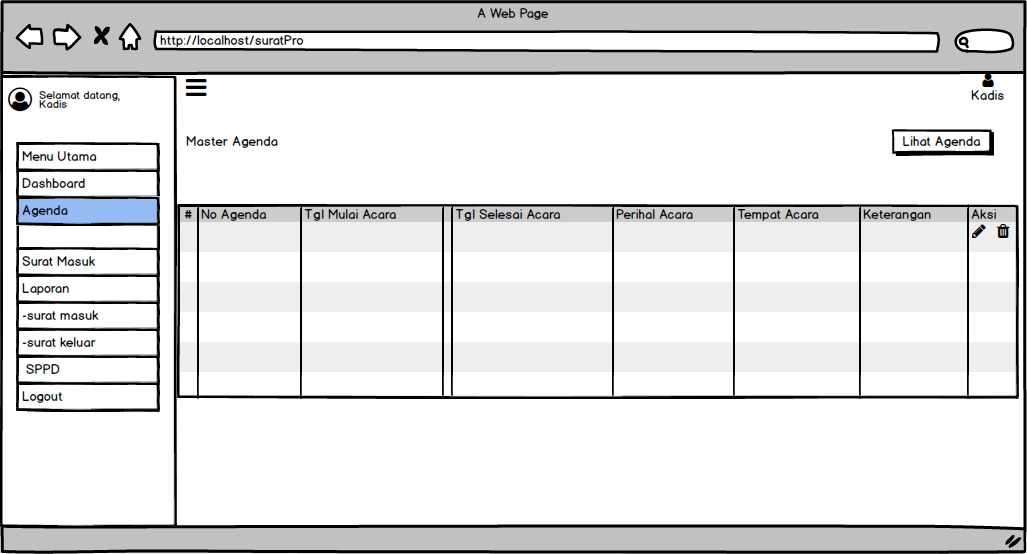
\includegraphics [height= 7cm, width=11cm]{konten/gambar/WireFrameSistemSurat/Kadis/DaftarAgenda.png}
			\caption{Halaman Lihat Daftar Agenda}
			\label{HalamanLihatDaftarAgendaKadis}
		\end{figure}
		
		\item Menu Master Jabatan
		
		Halaman Menu Master Golongan dapat dilihat pada \pic~\ref{HalamanLihatDaftarAgendaKadis}
		
		\begin{figure}
			\centering
			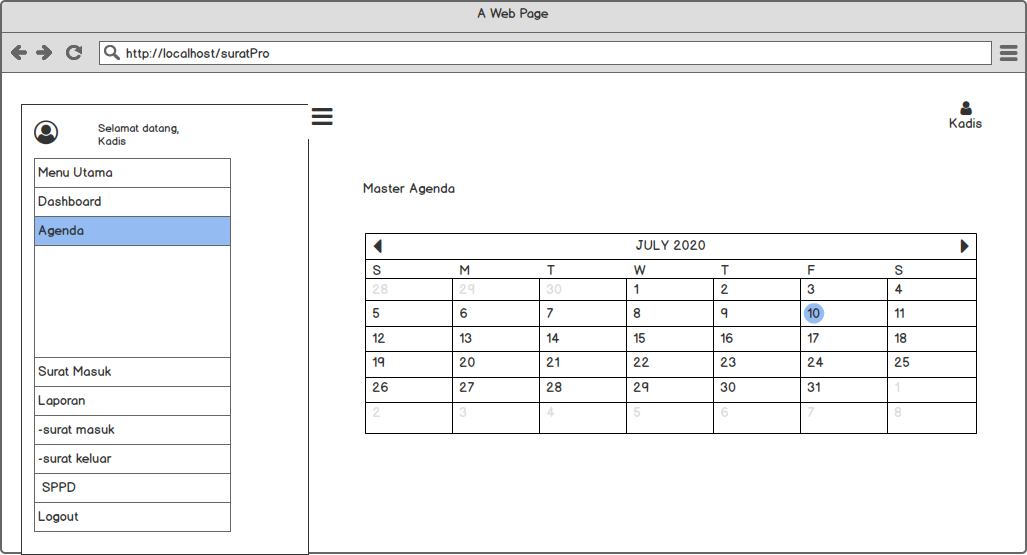
\includegraphics [height= 7cm, width=11cm]{konten/gambar/WireFrameSistemSurat/Kadis/TampilanAgendakalender.png}
			\caption{Tampilan Agenda Di Kalender}
			\label{HalamanTampilanAgendakalender}
		\end{figure}
		
		\item Menu Master Pegawai
		
		Halaman Menu Master Pegawai dapat dilihat pada \pic~\ref{HalamanSuratMasuk}
		
		\begin{figure}
			\centering
			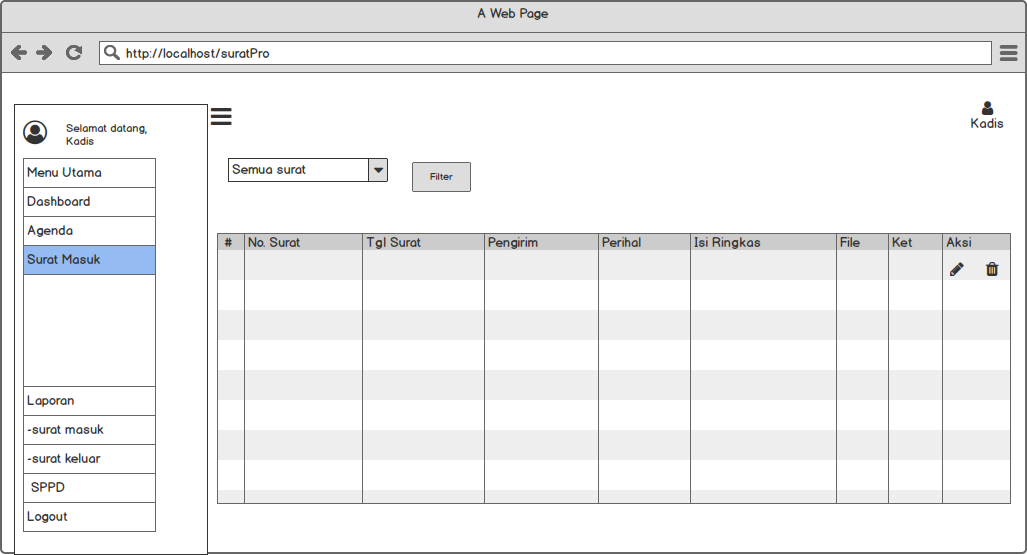
\includegraphics [height= 7cm, width=11cm]{konten/gambar/WireFrameSistemSurat/Kadis/SuratMasuk.png}
			\caption{Halaman Surat Masuk}
			\label{HalamanSuratMasuk}
		\end{figure}
		
		\item Menu Master Kategori Surat 
		
		Halaman Menu Master Kategori Surat dapat dilihat pada \pic~\ref{HalamanLaporanSuratMasukKadis}
		
		\begin{figure}
			\centering
			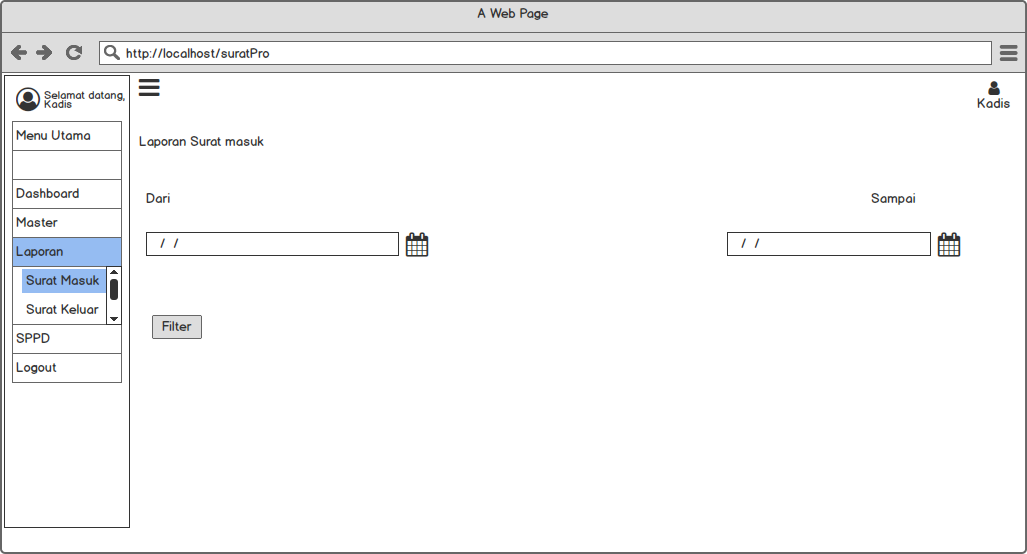
\includegraphics [height= 7cm, width=11cm]{konten/gambar/WireFrameSistemSurat/Kadis/LaporanSuratMasuk.png}
			\caption{Halaman Laporan Surat Masuk}
			\label{HalamanLaporanSuratMasukKadis}
		\end{figure}
		
		\item Menu Master Pengirim Surat
		
		Halaman Menu Master Pengirim Surat dapat dilihat pada \pic~\ref{HalamanLaporanSuratKeluar}
		
		\begin{figure}
			\centering
			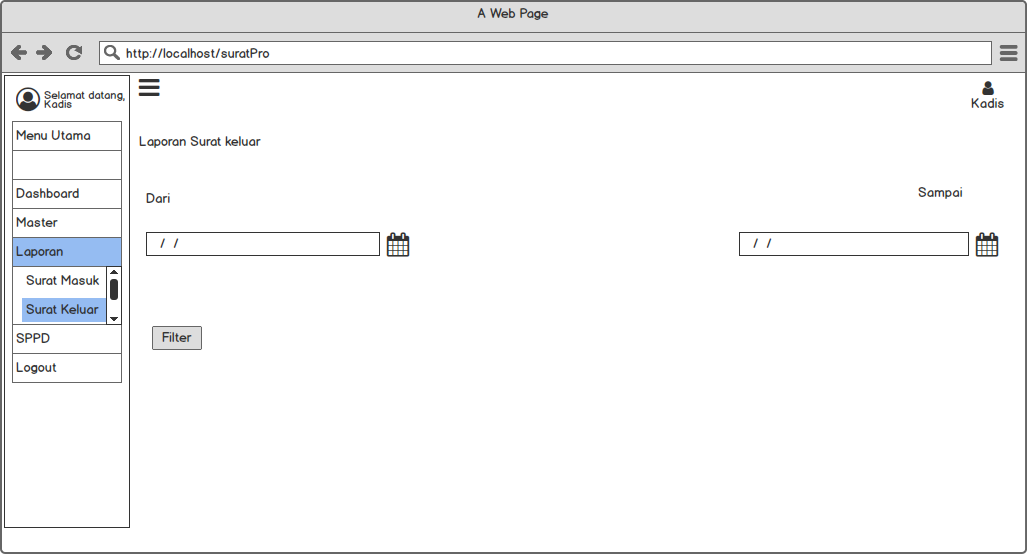
\includegraphics [height= 7cm, width=11cm]{konten/gambar/WireFrameSistemSurat/Kadis/LaporanSuratKeluar.png}
			\caption{Halaman Laporan Surat Keluar}
			\label{HalamanLaporanSuratKeluar}
		\end{figure}
		
		\item Menu SPPD Master Kegiatan
		
		Halaman Menu SPPD Master Kegiatan dapat dilihat pada \pic~\ref{HalamanLihatMasterSPPDKadis}
		
		\begin{figure}
			\centering
			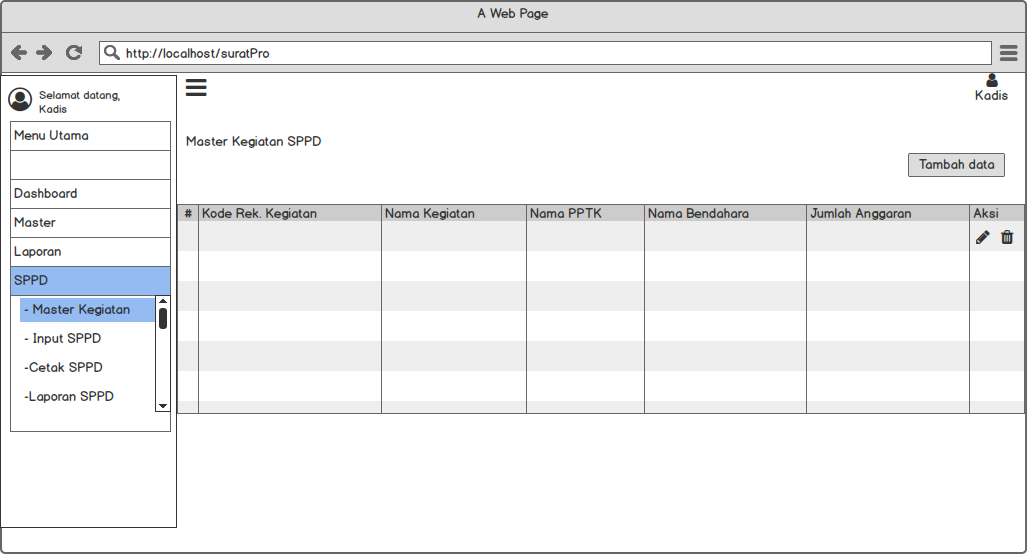
\includegraphics [height= 7cm, width=11cm]{konten/gambar/WireFrameSistemSurat/Kadis/MasterkegiatanSPPD.png}
			\caption{Halaman Lihat Master SPPD}
			\label{HalamanLihatMasterSPPDKadis}
		\end{figure}
		
		\item Menu SPPD Input SPPD
		
		Halaman Menu SPPD Input SPPD dapat dilihat pada \pic~\ref{HalamanInputMasterSPPDKadis}
		
		\begin{figure}
			\centering
			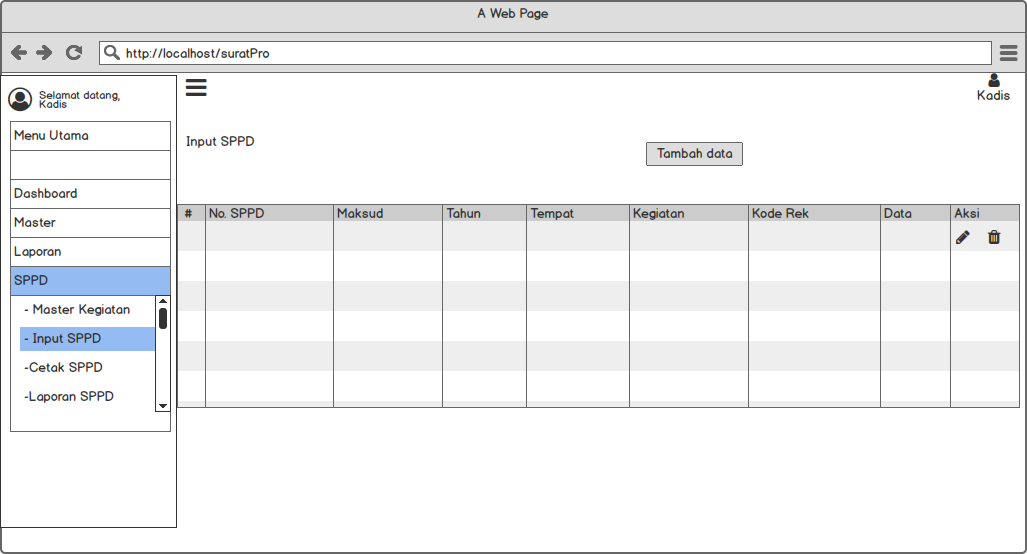
\includegraphics [height= 7cm, width=11cm]{konten/gambar/WireFrameSistemSurat/Kadis/InputSPPD.png}
			\caption{Halaman Input Master SPPD}
			\label{HalamanInputMasterSPPDKadis}
		\end{figure}
		
		\item Menu SPPD Cetak SPPD
		
		Halaman Menu SPPD Cetak SPPD dapat dilihat pada \pic~\ref{HalamanCetakSPPDKadis}
		
		\begin{figure}
			\centering
			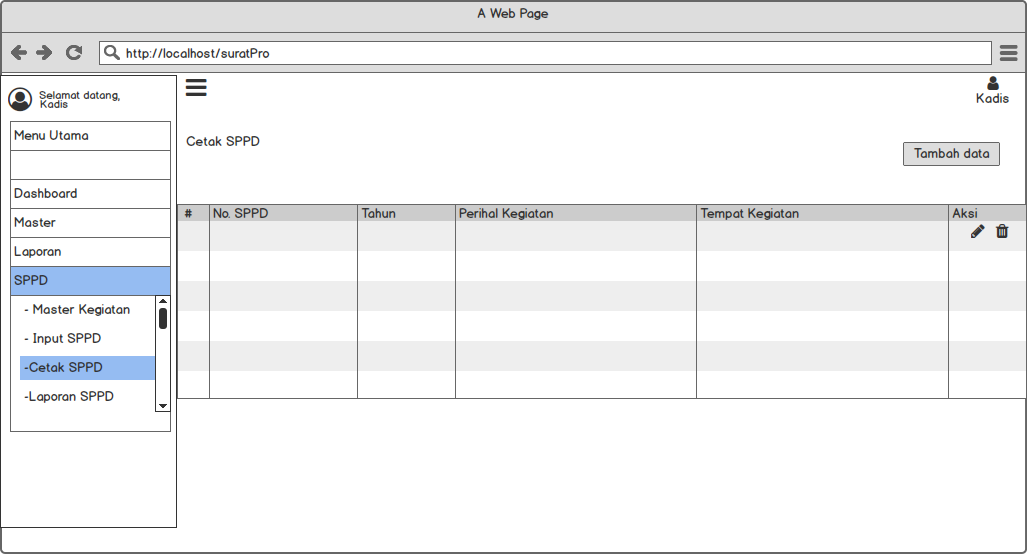
\includegraphics [height= 7cm, width=11cm]{konten/gambar/WireFrameSistemSurat/Kadis/CetakSPPD.png}
			\caption{Halaman Cetak SPPD}
			\label{HalamanCetakSPPDKadis}
		\end{figure}
		
		\item Menu Laporan SPPD
		
		Halaman Menu Laporan SPPD dapat dilihat pada \pic~\ref{HalamanLihatLaporanSPPDKadis}
		
		\begin{figure}
			\centering
			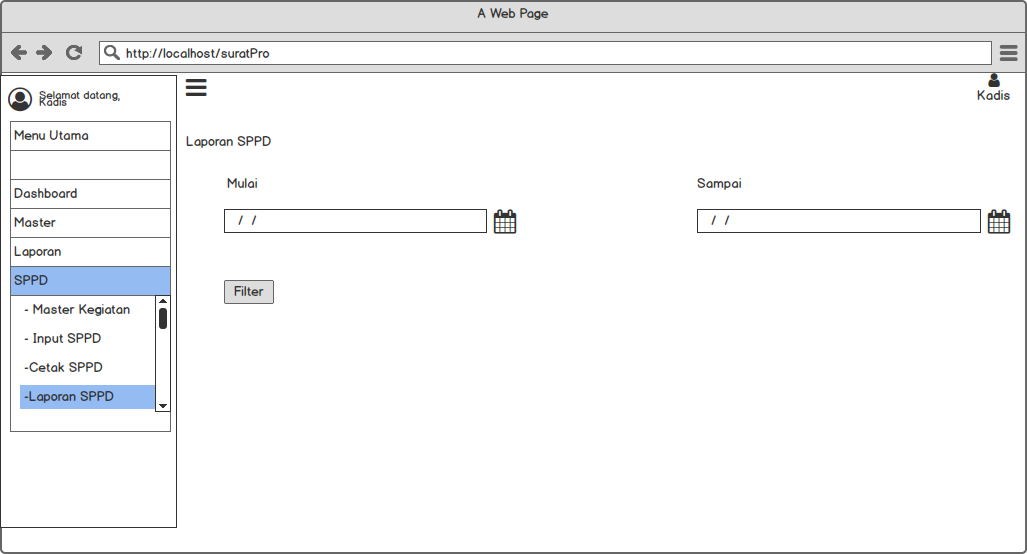
\includegraphics [height= 7cm, width=11cm]{konten/gambar/WireFrameSistemSurat/Kadis/LaporanSPPD.png}
			\caption{Halaman Lihat Laporan SPPD}
			\label{HalamanLihatLaporanSPPDKadis}
		\end{figure}
		
	\end{enumerate}
	
\item Desagin Antar Muka Pengagenda
	
	\begin{enumerate}
		\item Halaman Dashboard
		
		Halaman Desagin Dashboard dapat dilihat pada \pic~\ref{HalamanDashBoardPengagenda}
		
		\begin{figure}
			\centering
			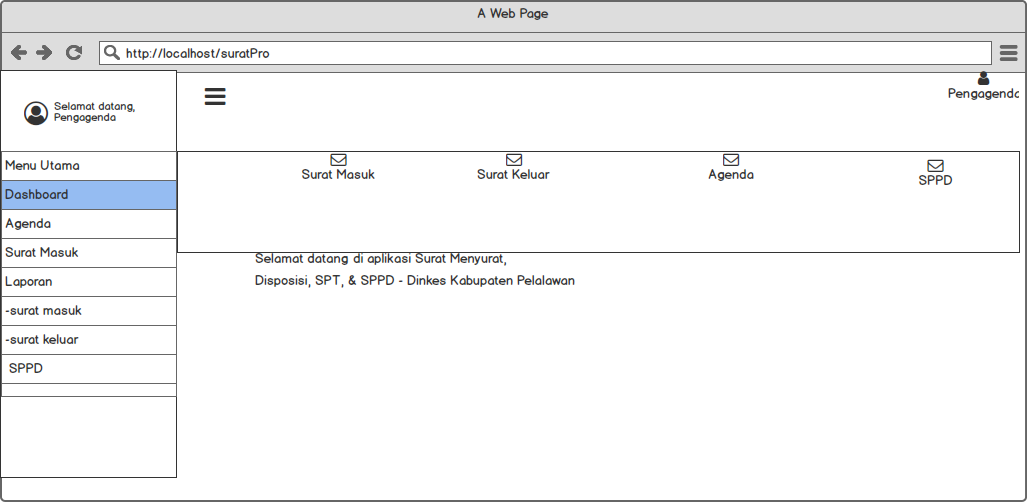
\includegraphics [height= 7cm, width=11cm]{konten/gambar/WireFrameSistemSurat/Pengagenda/DashBoard.png}
			\caption{Halaman DashBoard Pengagenda}
			\label{HalamanDashBoardPengagenda}
		\end{figure}
		
		\item Halaman Daftar Agenda
		
		Halaman Daftar Agenda dapat dilihat pada \pic~\ref{HalamanDaftarAgenda}.
		
		\begin{figure}
			\centering
			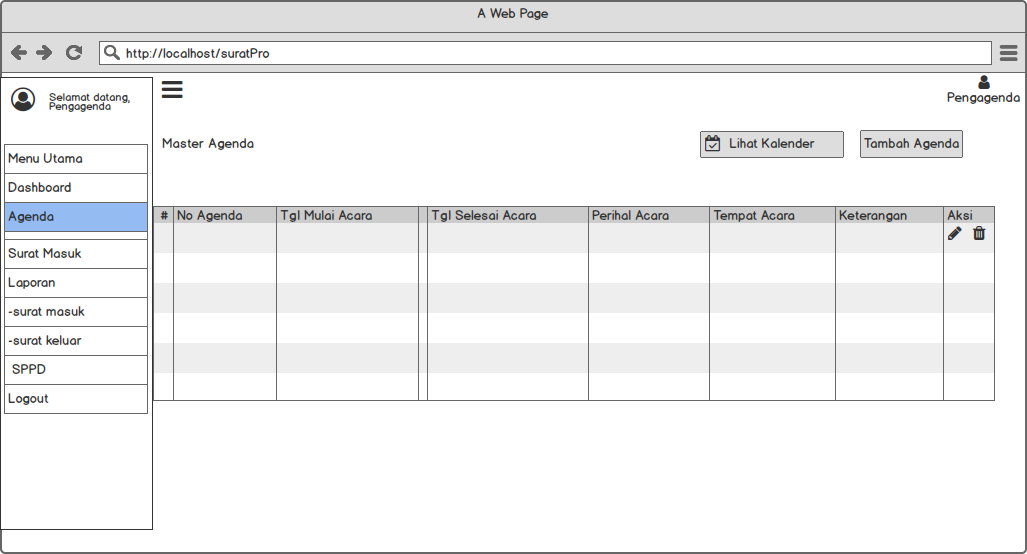
\includegraphics [height= 7cm, width=11cm]{konten/gambar/WireFrameSistemSurat/Pengagenda/DaftarAgenda.png}
			\caption{Halaman Daftar Agenda Pengagenda}
			\label{HalamanDaftarAgenda}
		\end{figure}
		
		\item Halaman Tampilan Agenda kalender Pengagenda
		
		Halaman Tampilan Agenda dapat dilihat pada \pic~\ref{HalamanTampilankalenderPengagenda}
		
		\begin{figure}
			\centering
			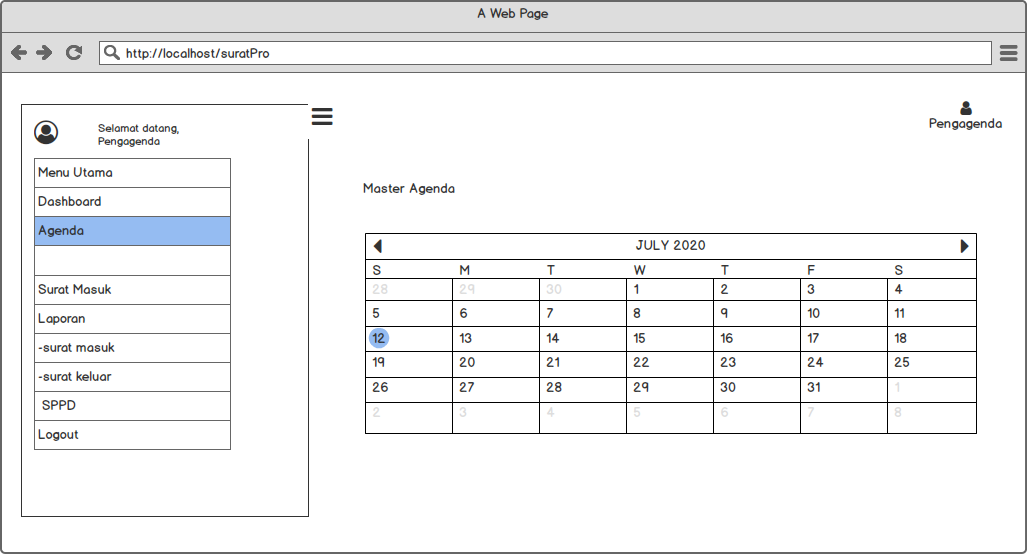
\includegraphics [height= 7cm, width=11cm]{konten/gambar/WireFrameSistemSurat/Pengagenda/TampilanAgendakalender.png}
			\caption{Halaman Tampilan Agenda kalender Pengagenda}
			\label{HalamanTampilankalenderPengagenda}
		\end{figure}
		
		\item Halaman Tampilan Tambah Agenda Kalender Pengagenda
		
		Halaman Tampilan Tambah Agenda Kalender Pengagenda dapat dilihat pada \pic~\ref{TampilanTambahAgendakalenderPenagenda}
		
		\begin{figure}
			\centering
			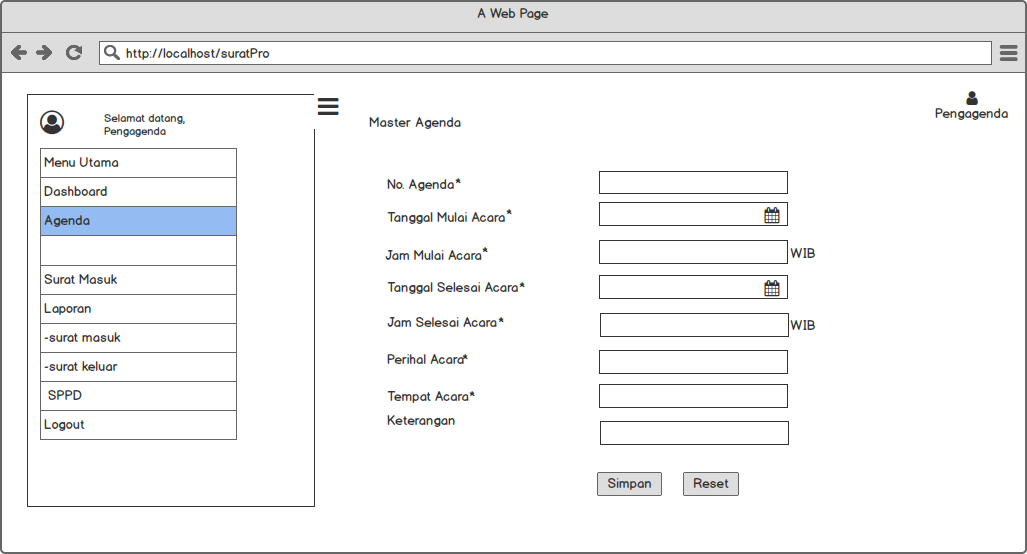
\includegraphics [height= 7cm, width=11cm]{konten/gambar/WireFrameSistemSurat/Pengagenda/TampilanTambahAgendakalender.png}
			\caption{Halaman Tampilan Tambah Agenda Kalender Pengagenda}
			\label{TampilanTambahAgendakalenderPenagenda}
		\end{figure}
		
		\item Halaman Surat Masuk Pengagenda
		
		Halaman Halaman Surat Masuk Pengagenda dapat dilihat pada \pic~\ref{HalamanSuratMasukPengagenda}
		
		\begin{figure}
			\centering
			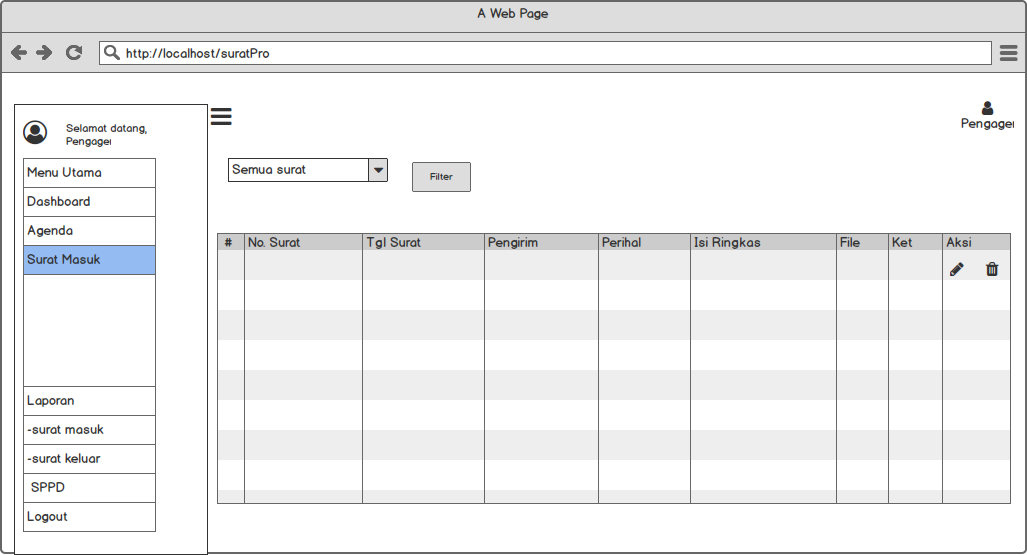
\includegraphics [height= 7cm, width=11cm]{konten/gambar/WireFrameSistemSurat/Pengagenda/SuratMasuk.png}
			\caption{Halaman Surat Masuk Pengagenda}
			\label{HalamanSuratMasukPengagenda}
		\end{figure}
		
		\item Halaman Laporan Surat Masuk Pengagenda
		
		Halaman Laporan Surat Masuk Pengagenda dapat dilihat pada \pic~\ref{HalamanLaporanSuratMasukPengagenda}
		
		\begin{figure}
			\centering
			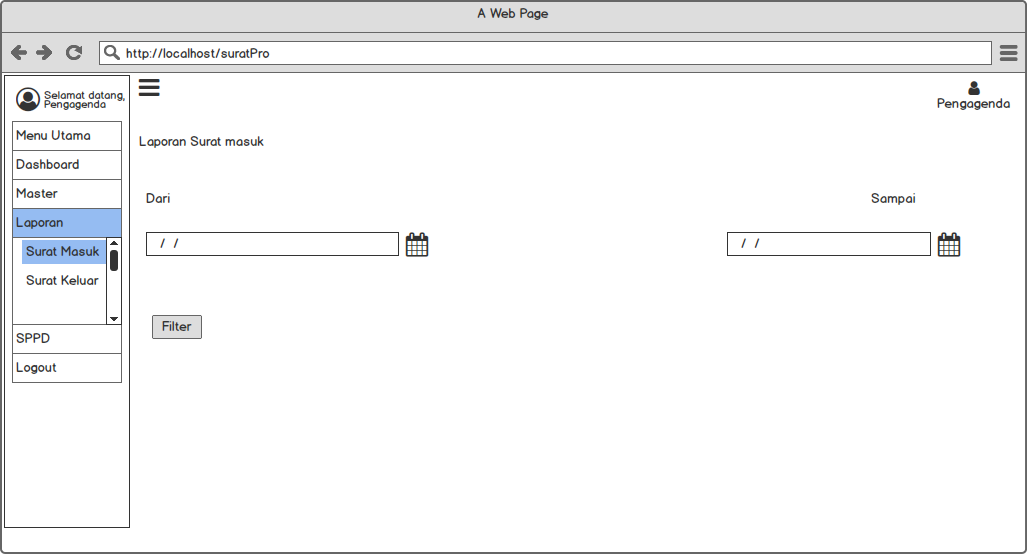
\includegraphics [height= 7cm, width=11cm]{konten/gambar/WireFrameSistemSurat/Pengagenda/LaporanSuratMasuk.png}
			\caption{Halaman Laporan Surat Masuk Pengagenda}
			\label{HalamanLaporanSuratMasukPengagenda}
		\end{figure}
		
		\item Halaman Laporan Surat Keluar Pengagenda
		
		Halaman Laporan Surat Keluar Pengagenda dapat dilihat pada \pic~\ref{LaporanSuratKeluarPengagenda}
		
		\begin{figure}
			\centering
			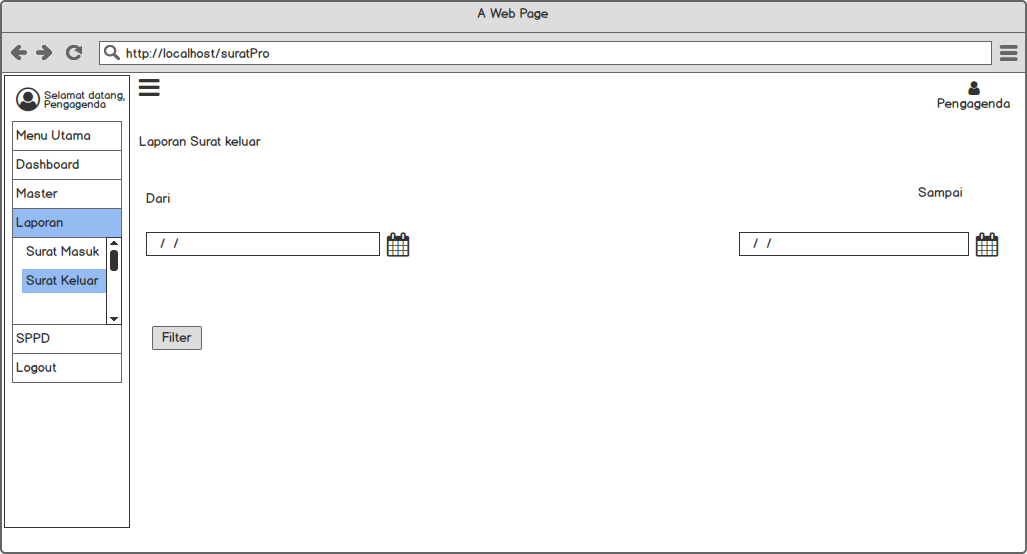
\includegraphics [height= 7cm, width=11cm]{konten/gambar/WireFrameSistemSurat/Pengagenda/LaporanSuratKeluar.png}
			\caption{Halaman Laporan Surat Keluar Pengagenda}
			\label{LaporanSuratKeluarPengagenda}
		\end{figure}
		
		\item Halaman Lihat Master SPPD Pengagenda
		
		Halaman Lihat Master SPPD Pengagenda dapat dilihat pada \pic~\ref{HalamanLihatMasterSPPDPengagenda}
		
		\begin{figure}
			\centering
			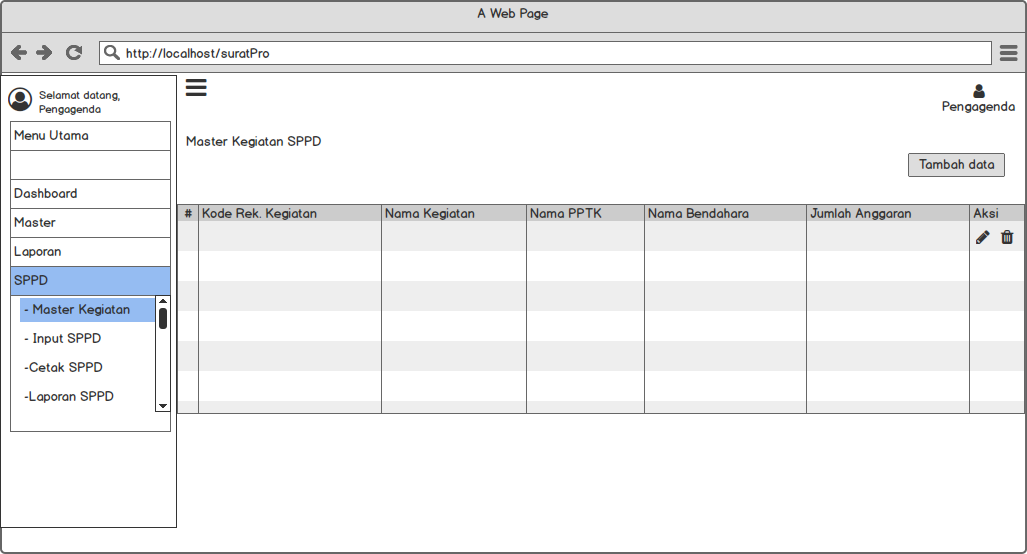
\includegraphics [height= 7cm, width=11cm]{konten/gambar/WireFrameSistemSurat/Pengagenda/MasterkegiatanSPPD.png}
			\caption{Halaman Lihat Master SPPD Pengagenda}
			\label{HalamanLihatMasterSPPDPengagenda}
		\end{figure}
		
		\item Halaman Input Master SPPD Pengagenda
		
		Halaman Input Master SPPD Pengagenda dapat dilihat pada \pic~\ref{HalamanInputMasterSPPDPengagenda}
		
		\begin{figure}
			\centering
			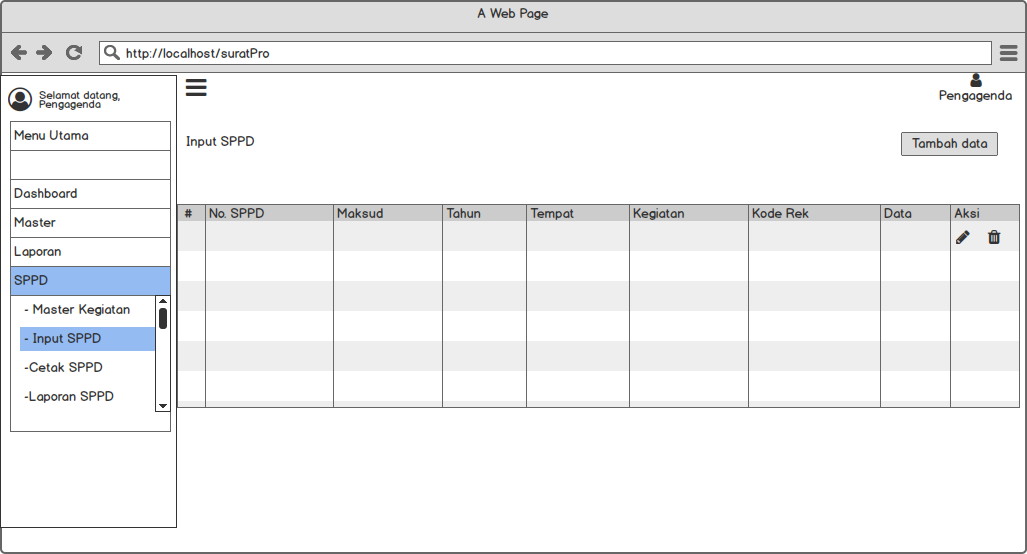
\includegraphics [height= 7cm, width=11cm]{konten/gambar/WireFrameSistemSurat/Pengagenda/InputSPPD.png}
			\caption{Halaman Input Master SPPD Pengagenda}
			\label{HalamanInputMasterSPPDPengagenda}
		\end{figure}
		
		\item Halaman Cetak SPPD Pengagenda
		
		Halaman Cetak SPPD Pengagenda dapat dilihat pada \pic~\ref{HalamanCetakSPPDPengagenda}
		
		\begin{figure}
			\centering
			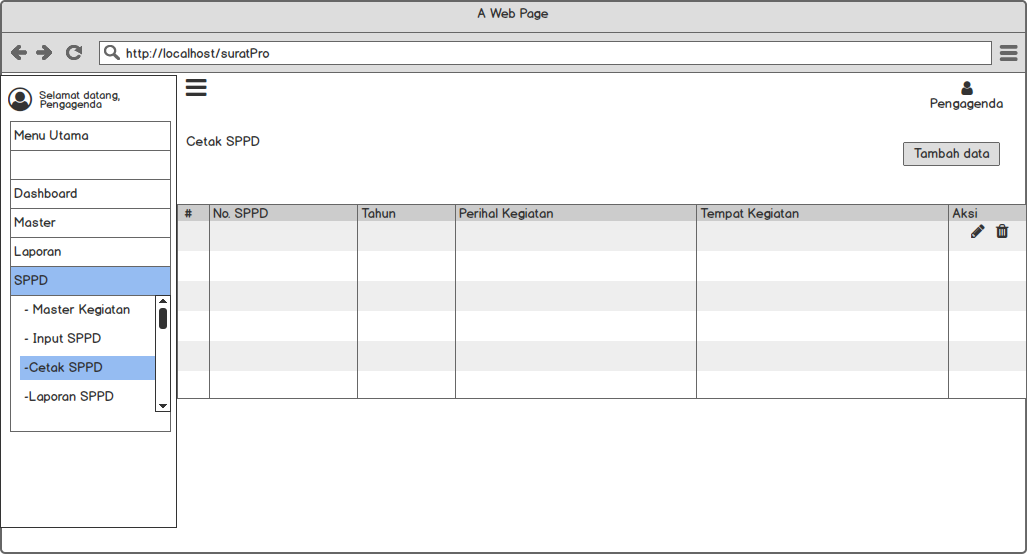
\includegraphics [height= 7cm, width=11cm]{konten/gambar/WireFrameSistemSurat/Pengagenda/CetakSPPD.png}
			\caption{Halaman Cetak SPPD Pengagenda}
			\label{HalamanCetakSPPDPengagenda}
		\end{figure}
		
		\item Halaman Cetak SPPD Pengagenda
		
		Halaman Cetak SPPD Pengagenda dapat dilihat pada \pic~\ref{HalamanLaporanSPPDPengagenda}
		
		\begin{figure}
			\centering
			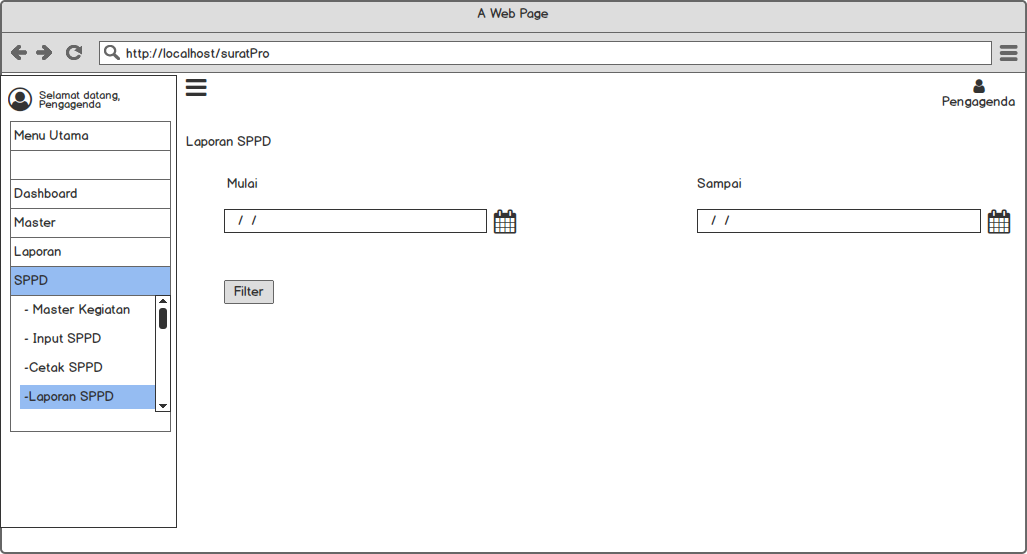
\includegraphics [height= 7cm, width=11cm]{konten/gambar/WireFrameSistemSurat/Pengagenda/LaporanSPPD.png}
			\caption{Halaman Cetak SPPD Pengagenda}
			\label{HalamanLaporanSPPDPengagenda}
		\end{figure}
		
	\end{enumerate}
	
	\item Desaign Antar Muka Pegawai
	
	\begin{enumerate}
		\item Halaman dashboard
		
		Halaman dashboard dapat dilihat pada \pic~\ref{HalamanDashBoardPegawai}
		
		\begin{figure}
			\centering
			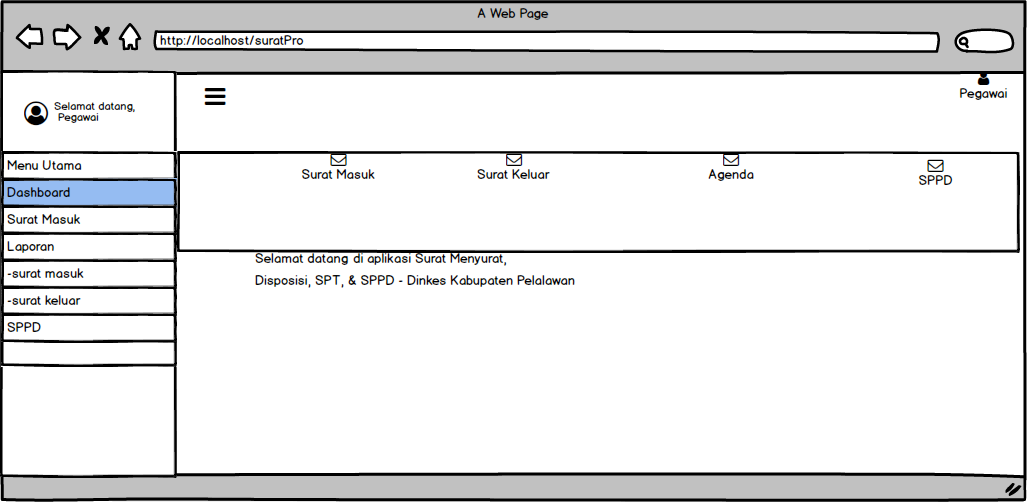
\includegraphics [height= 7cm, width=11cm]{konten/gambar/WireFrameSistemSurat/Pegawai/DashBoard.png}
			\caption{Halaman DashBoard Pegawai}
			\label{HalamanDashBoardPegawai}
		\end{figure}
		
		\item Halaman Surat Masuk
		
		Halaman Surat Masuk dapat dilihat pada \pic~\ref{HalamanSuratMasukPegawai}
		
		\begin{figure}
			\centering
			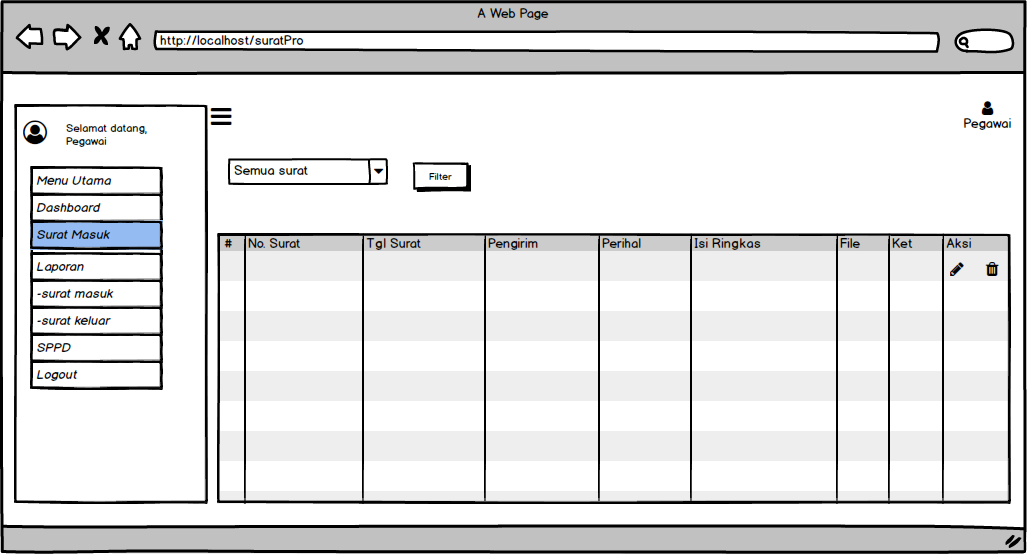
\includegraphics [height= 7cm, width=11cm]{konten/gambar/WireFrameSistemSurat/Pegawai/SuratMasuk.png}
			\caption{Halaman Surat Masuk Pegawai}
			\label{HalamanSuratMasukPegawai}
		\end{figure}
		
		\item Laporan Surat Masuk
		
		Laporan Surat Masuk dapat dilihat pada \pic~\ref{HalamanLaporanSuratMasukPegawai}
		
		\begin{figure}
			\centering
			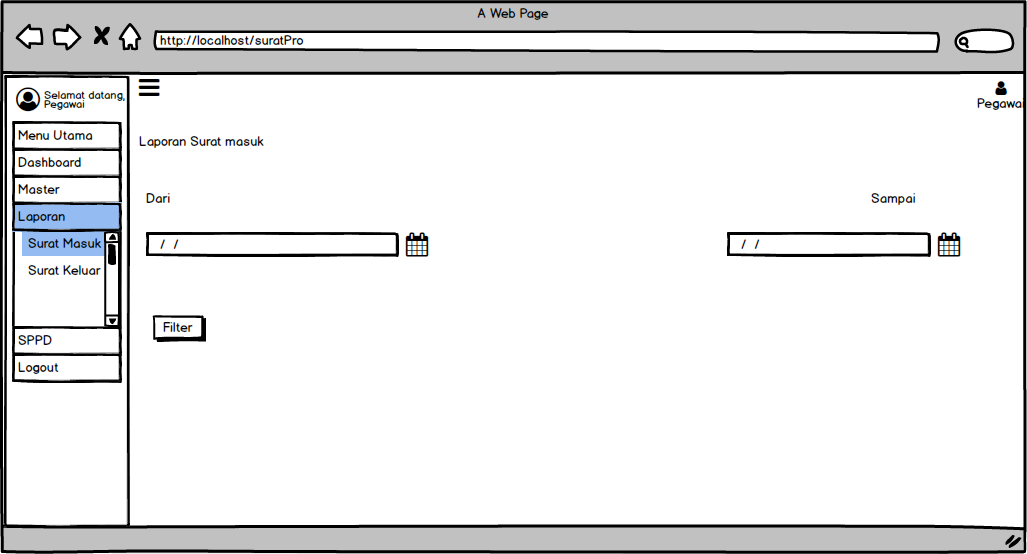
\includegraphics [height= 7cm, width=11cm]{konten/gambar/WireFrameSistemSurat/Pegawai/LaporanSuratMasuk.png}
			\caption{Halaman Laporan Surat Masuk Pegawai}
			\label{HalamanLaporanSuratMasukPegawai}
		\end{figure}
		
		\item Laporan Surat Keluar
		
		Laporan Surat Keluar dapat dilihat pada \pic~\ref{HalamanLaporanKeluarMasukPegawai}
		
		\begin{figure}
			\centering
			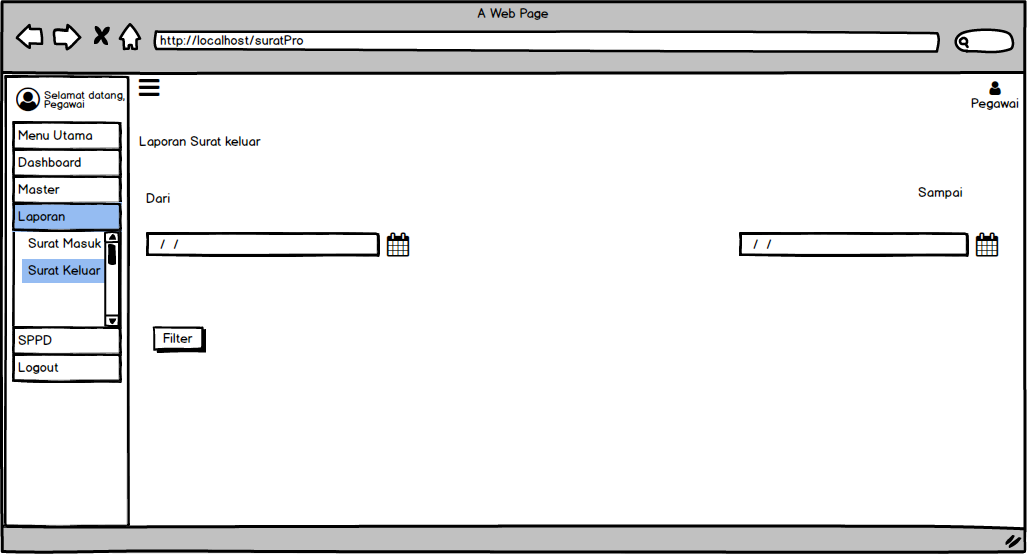
\includegraphics [height= 7cm, width=11cm]{konten/gambar/WireFrameSistemSurat/Pegawai/LaporanSuratKeluar.png}
			\caption{Halaman Laporan Surat Masuk Pegawai}
			\label{HalamanLaporanKeluarMasukPegawai}
		\end{figure}
		
		\item Laporan Master SPPD 
		
		Laporan Master SPPD dapat dilihat pada \pic~\ref{HalamanMasterkegiatanSPPDPegawai}
		
		\begin{figure}
			\centering
			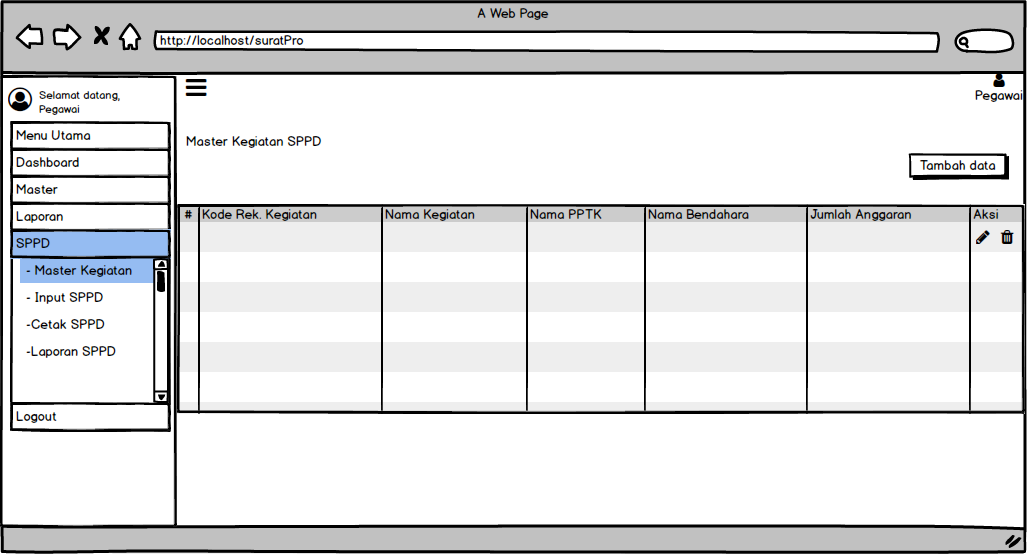
\includegraphics [height= 7cm, width=11cm]{konten/gambar/WireFrameSistemSurat/Pegawai/MasterkegiatanSPPD.png}
			\caption{Halaman Master kegiatan SPPD Pegawai}
			\label{HalamanMasterkegiatanSPPDPegawai}
		\end{figure}
		
		\item Laporan Input SPPD 
		
		Laporan Input SPPD  dapat dilihat pada \pic~\ref{HalamanHalamanInputSPPDPegawai}
		
		\begin{figure}
			\centering
			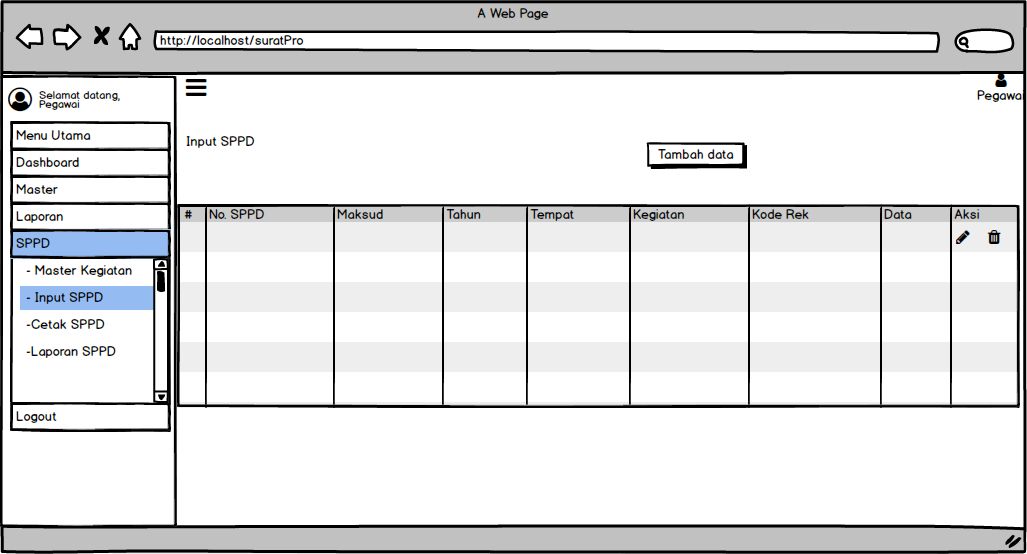
\includegraphics [height= 7cm, width=11cm]{konten/gambar/WireFrameSistemSurat/Pegawai/InputSPPD.png}
			\caption{Halaman Input SPPD Pegawai}
			\label{HalamanHalamanInputSPPDPegawai}
		\end{figure}
		
		\item Laporan Cetak SPPD 
		
		Laporan Cetak SPPD dapat dilihat pada \pic~\ref{HalamanCetakSPPDPegawai}
		
		\begin{figure}
			\centering
			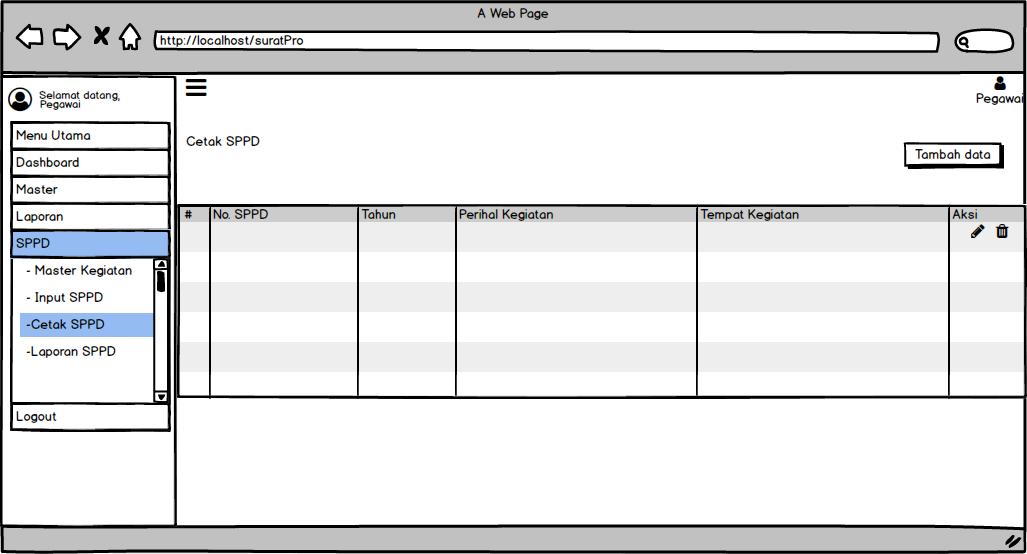
\includegraphics [height= 7cm, width=11cm]{konten/gambar/WireFrameSistemSurat/Pegawai/CetakSPPD.png}
			\caption{Halaman Cetak SPPD Pegawai}
			\label{HalamanCetakSPPDPegawai}
		\end{figure}
		
		\item Laporan SPPD 
		
		Halaman Laporan SPPD  dapat dilihat pada \pic~\ref{HalamanLaporanSPPDPegawai}
		
		\begin{figure}
			\centering
			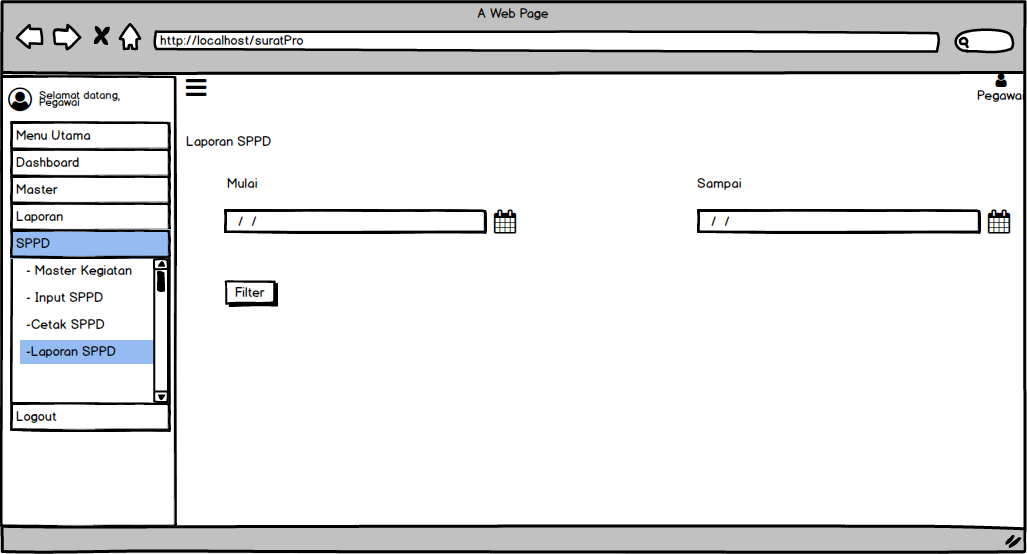
\includegraphics [height= 7cm, width=11cm]{konten/gambar/WireFrameSistemSurat/Pegawai/LaporanSPPD.png}
			\caption{Halaman Laporan SPPD Pegawai}
			\label{HalamanLaporanSPPDPegawai}
		\end{figure}
	\end{enumerate}
\end{enumerate}

